\documentclass{beamer}
\usepackage{bm}
\usepackage{listings}

\usepackage{tikz}
\usepackage{svn_latex/hybtikz}
%\usetikzlibrary{arrows}
\usetikzlibrary{arrows}
\usepackage{bm}
\usepackage[utf8]{inputenc}
%\usepackage{listings}
\usepackage{minted}
\usepackage[english]{babel}
\usepackage{amsmath}
\usepackage{stmaryrd}
\usepackage{mathrsfs}
\usepackage{multimedia}
\lstset{basicstyle=\footnotesize}


\usepackage{algorithm}
\usepackage{algorithmic}
%\usepackage{verbatim}

% \lstloadlanguages{C}
% \lstset{language=C}
% columns=flexible, basicstyle=\footnotesize\sffamily, keywordstyle=\color{motcle}\bfseries,identifierstyle=\color{ocre}\itshape,stringstyle=\color{blue},commentstyle=\color{vert}}


% \lstset{basicstyle=\footnotesize}



\setminted[python]{
  style=vs,
  fontsize=\footnotesize,
  frame=single,
  breaklines=true,
  linenos=false
}

\setbeamertemplate{navigation symbols}{}
\setbeamertemplate{footline}{}


\title{Machine Learning for Business}
\author{ Thibault Defourneau, Mihaly Petrecky \\ 
defourneau.thibault@gmail.com, mihaly.petreczky-ext@skema.edu }


\begin{document}
\begin{frame}\maketitle\end{frame}


\begin{frame}{Key Points of the Course}

\textbf{Objective}

\begin{itemize}
    \item Understand the core principles of Machine Learning
    \item Connect theory to real business decision-making
\end{itemize}

\vspace{0.4cm}

\textbf{Learning Outcomes}

\begin{itemize}
    \item Select appropriate models depending on the problem
    \item Interpret results and evaluate performance
    \item Understand limitations and trade-offs
\end{itemize}

\vspace{0.4cm}

\textbf{Assessment \& Practice}

\begin{itemize}
    \item Applied exercises throughout the course
    \item Mid-term exam (March 10th)
    \item Final group business project
\end{itemize}

\end{frame}


% =====================================================

\begin{frame}
\frametitle{Course Roadmap — Machine Learning for Business}

\tableofcontents
\end{frame}

% =====================================================


% =====================================================
\section{Module 0 — Big Picture of Machine Learning}

\begin{frame}{Module 0 — Big Picture}
\begin{itemize}
    \item What is Machine Learning?
    \item Supervised vs Unsupervised Learning
    \item From Data to Decision-Making
\end{itemize}
\end{frame}

\begin{frame}{What is Machine Learning?}
\textbf{Definition:} Machine Learning (ML) enables algorithms to learn patterns and tasks directly from data without being explicitly programmed.

\vspace{0.5cm}

\textbf{Key Points:}
\begin{itemize}
    \item ML lies at the intersection of \textbf{Mathematics} and \textbf{Computer Science}.
    \item A \textbf{Machine Learning Model} automates repetitive tasks.
    \item An \textbf{AI Agent} goes further: it takes decisions and actions based on triggers and observations.
    \item Two main strategies to teach a Machine Learning Model:
    \begin{itemize}
        \item \textit{Supervised Learning}: The model is guided using labeled data points $(x_i, y_i)$.
        \item \textit{Unsupervised Learning}: The model discovers structure or patterns in unlabeled data $(x_i)$.
    \end{itemize}
\end{itemize}

\end{frame}

\begin{frame}{Supervised Learning}
\textbf{Setup:} We have input-output pairs:

\[
(x_i, y_i), \quad i=1,\dots,n
\]

\textbf{Goal:} Learn a function $f(x)$ that predicts $y$ accurately.

\vspace{0.5cm}

\textbf{Two main types:}
\begin{itemize}
    \item \textit{Regression:} Predict a continuous outcome (e.g., house prices, sales forecast)
    \item \textit{Classification:} Predict a categorical outcome (e.g., loan default, churn yes/no)
\end{itemize}

\vspace{0.5cm}

\textbf{Business Example:}  
A bank wants to predict whether a new applicant will default (classification) or estimate the expected loan amount (regression).
\end{frame}

\begin{frame}{Unsupervised Learning}
\textbf{Goal:} Discover structure in unlabeled data.

\vspace{0.5cm}

We observe only features:

\[
x_i, \quad i=1,\dots,n
\]

No target $y$ is available.

\vspace{0.5cm}

\textbf{Common Tasks:}
\begin{itemize}
    \item \textit{Clustering}: Group similar data points (e.g., customer segmentation)
    \item \textit{Dimensionality Reduction}: Summarize data with fewer variables (e.g., PCA for marketing analytics)
\end{itemize}

\vspace{0.5cm}

\textbf{Business Example:}  
A retail company wants to identify customer segments based on purchase behavior to design targeted marketing campaigns.
\end{frame}

\begin{frame}{Data-Driven Approach}
\textbf{Idea:} Use data to drive business decisions instead of intuition alone.

\vspace{0.5cm}

\textbf{Steps:}
\begin{enumerate}
    \item Collect and clean relevant data
    \item Explore and visualize patterns
    \item Build predictive or descriptive models
    \item Make decisions and take action
    \item Monitor outcomes and iterate
\end{enumerate}

\vspace{0.5cm}

\textbf{Business Example:}  
A bank wants to optimize credit offers:
\begin{itemize}
    \item Analyze past customer data
    \item Predict likelihood of accepting a new offer
    \item Adjust campaigns dynamically
\end{itemize}

\end{frame}


% =====================================================
\section{Module 1 — Probability and Statistical Foundations}

\begin{frame}{Module 1 — Probability Foundations}
\begin{itemize}
    \item Random Variables (Discrete and Continuous)
    \item Probability Distributions
    \item Expectation and Variance
    \item Normal Distribution
    \item Law of Large Numbers
    \item Central Limit Theorem
    \item Confidence Intervals
    \item Bayes’ Theorem
\end{itemize}
\end{frame}

\begin{frame}{Why Probability in Business?}

\textbf{Business Example: Loan Default}

A bank evaluates loan applications.

\begin{itemize}
    \item 8\% of all customers default
    \item 25\% of customers with low credit score default
\end{itemize}

\vspace{0.3cm}

\textbf{Question:}
\begin{center}
What is the probability that a new applicant will default?
\end{center}

\vspace{0.5cm}

\textbf{Key Idea:} Business decisions are made under uncertainty.

\end{frame}
\begin{frame}{Why We Need Probability in Machine Learning}

In machine learning, we try to predict an output based on input variables such as 
education, experience, age, or other business characteristics.

\medskip

\textbf{However, in real life the same inputs do not always lead to the same output.}

\begin{itemize}
    \item Two people with the same education and experience may earn different wages.
    \item Two customers with identical profiles may behave differently.
    \item Two products with the same features may still sell at different prices.
\end{itemize}

\medskip

This variation comes from many sources:

\begin{itemize}
    \item unobserved factors,
    \item randomness in human behaviour,
    \item measurement errors,
    \item missing information,
    \item natural economic and social variability.
\end{itemize}

\end{frame}


\begin{frame}{Why Probability Is Necessary}

Because outcomes vary even when inputs are identical, machine learning models must
treat outputs as \textbf{random variables} rather than fixed quantities.

\medskip

Your probability tools explain how to describe such randomness:

\begin{itemize}
    \item A random variable represents all possible outcomes.
    \item Probability tells us how frequently each outcome occurs.
    \item Expected value describes the long-run average.
    \item Variance measures uncertainty and risk.
    \item The Law of Large Numbers explains why estimates improve with more data.
    \item The Central Limit Theorem explains why averages behave predictably.
\end{itemize}

\end{frame}


\begin{frame}{Probability and Model Evaluation}

Probability theory is essential for understanding and evaluating machine learning
models:

\begin{itemize}
    \item It explains why models cannot predict perfectly.
    \item It allows us to estimate and interpret prediction errors.
    \item It provides the foundation for loss functions used in training.
    \item It helps us understand how models generalize to unseen data.
    \item It quantifies uncertainty in business predictions.
\end{itemize}

\medskip

\textbf{Machine learning does not predict exact outcomes.  
It predicts patterns in data that are inherently variable.  
Probability allow us to evaluate these predictions.}

\end{frame}
\begin{frame}{Set of all outcomes $\Omega$}

We imagine an Excel file containing rows such as:
experience, education, wage, gender, etc.

\medskip

If more people are observed, the file grows: each new person adds a new row.

\medskip

\textbf{$\Omega$ is defined as the collection of all possible rows}
that could ever appear in this Excel file.

\medskip

In \textbf{general:} $\Omega$ is the collection of all possible rows. 

\medskip

Each row in our dataset is one observed element of $\Omega$.
Future data are simply additional elements drawn from the same set.

\end{frame}
\begin{frame}{Probability measure}

%\begin{itemize}
%    \item $\Omega$ is the set of all possible rows of the Excel file  
%          (all possible combinations of experience, education, wage, gender, etc.).
%    \item Each observed row is one element $\omega \in \Omega$.
%\end{itemize}


%\medskip 

Probability describes how often different types of rows appear.

\medskip

A \textbf{event} $A$ is a subset of $\Omega$: collection of rows with a certain property: certain combination of values of columns. 

\textbf{Examples of probability events:}
\begin{itemize}
    \item Wage smaller than 10.
    \item Education greater than 8.
    \item Female = 1 (the worker is female).
    \item ``Female = 1 AND education $> 8$ AND wage $< 10$.''
\end{itemize}

\medskip

 \textbf{Probability $P(A)$ of an event $A$}: how often we see rows from $A$
 
\end{frame}
\begin{frame}{Probability $P(A)$ of an event $A$: a more precise defintion}

  Choose $N$ rows from $\Omega$, $N$ large

 \[ P(A)=\frac{\mbox{number of rows among the chosen $N$ rows which are in $A$}}{N} \]


  We want $P(A)$ to be roughly the same as $N$ grows: limit exists

 \[ P(A)=\lim_{N \rightarrow \infty} \frac{\mbox{number of rows among the chosen $N$ rows which are in $A$}}{N} \]


 \medskip

 The elements of $\Omega$ should be \textbf{independent samples}: the frequencies
  \[ \frac{\mbox{number of rows among the chosen $N$ rows which are in $A$}}{N} \]
  should be approximately for the same $N$ for any choice of $N$ rows.

  \medskip
   If rows correspond to time (time-series), not always true. 



\end{frame}
\begin{frame}{Probability: difficulties}
  
    The precise definition is difficult: Kolmogorov 1930's, advanced math.
    
\textbf{Properties:}
\begin{itemize}
    \item $P(A) \ge 0$ for all events $A$,
    \item $P(\Omega) = 1$,
    \item If $A$ and $B$ cannot occur at the same time,  
          then $P(A \cup B) = P(A) + P(B)$.
\end{itemize}

\bigskip

\textbf{Probability is not always defined}
   The frequency 
  \[ \frac{\mbox{number of rows among the chosen $N$ rows which are in $A$}}{N} \]

  need not stabilize as $N$ grows. 

 \medskip

 We can never know based on data if probability is defined, we assume it. 

 \medskip

 We can make some experiments to see if this assumption is not invalidated.


\end{frame}
\begin{frame}{Random variable}
A \textbf{random variable} assigns a numerical value to every row in $\Omega$.

\medskip

Formally:
\[
X: \Omega \to \mathbb{R}
\]

\medskip

\textbf{Interpretation:}
\begin{itemize}
    \item Each column in the Excel file is a random variable.
    \item The random variable takes a row and outputs the value in that column.
\end{itemize}

\medskip

Examples:
\begin{itemize}
    \item Experience: maps each row to that person's experience.
    \item Education: maps each row to that person's education.
    \item Wage: maps each row to that person's wage.
    \item Gender: maps each row to 0 (male) or 1 (female).
\end{itemize}

\end{frame}
\begin{frame}{Discrete and Continuous Random Variables}

A random variable can have two types of possible values:

\medskip

\textbf{Discrete random variables}
\begin{itemize}
    \item Take values like 0, 1, 2, 3, ...
    \item There are no values in between.
    \item Example: gender (0 = male, 1 = female).
\end{itemize}

\medskip

\textbf{Continuous random variables}
\begin{itemize}
    \item Can take any value with decimals in between.
    \item Example: wage (10.2, 10.21, 10.212, and so on).
\end{itemize}

\medskip

The value of a random variable for a given row  
depends on the values in that row's columns.

\end{frame}


\begin{frame}{Probability Distributions}

A probability distribution describes how the values of a random
variable are spread across all possible rows in $\Omega$.

\medskip

\textbf{Discrete case $p(a)$:} event $X=a$ -- all rows to which $X$  assigns $a$. 
 \[ p(a)=\mathbf{P}(X=a) \]
 
$p(a)$ is relative frequency of rows for which $X$ is  $a$.

\textbf{Continuous case $F(a)$:}
  Events:$X \le a$, $X \ge b$.
  \[ F(a) = \mathbf{P}(X \le  a )\]

    $F(a)$ is relative frequency of rows for which $X \le a$.
        
  
  \[  \mathbf{P}(a \le X \le  b) = \left\{\begin{array}{rl} \sum_{s=a}^{b}
     p(s) & \mbox{ discrete } \\
    F(b)-F(a) & \mbox{ continuous }
  \end{array}\right.
  \]


%Thus, the distribution of a random variable depends entirely on the
%relative frequencies of certain combinations of column values in $\Omega$.

\end{frame}
\begin{frame}{Probability Density Function}

\textbf{Definition:}
A continuous random variable has a density $f(x)$ such that:

\begin{itemize}
    \item $f(x) \ge 0$
    \item $\int_{-\infty}^{\infty} f(x)\, dx = 1$
    \item $f$ is the derivative of the probability distribution 
         $\frac{dF(a)}{da}=f(a)$.
\end{itemize}

\vspace{0.5cm}

\textbf{Probability of an interval:}

\[
\mathbf{P}(a \le X \le b)
=
\int_a^b f(x)\, dx
\]

\end{frame}
\begin{frame}
  $f$ - density function.  Integral: area under curve. 




\begin{center}
 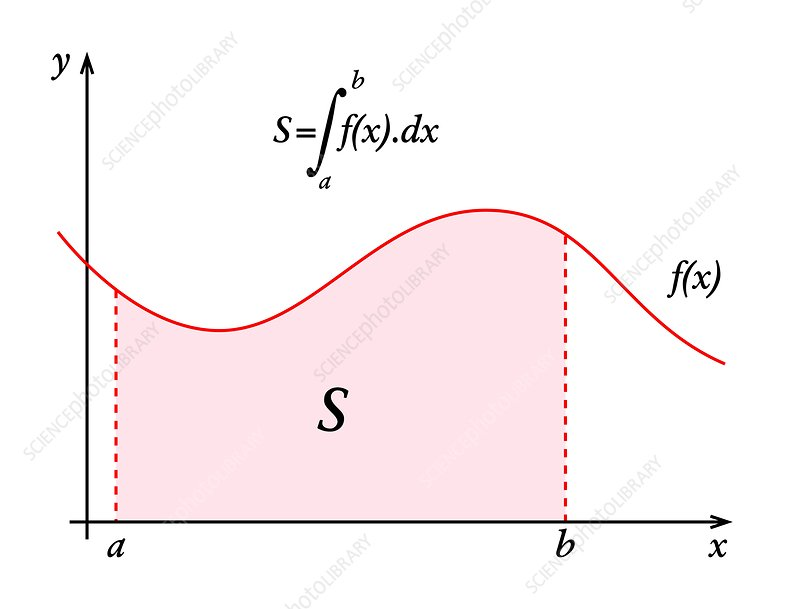
\includegraphics[scale=0.2]{integral.jpeg} 
\end{center}


\end{frame}
\begin{frame}{Example of density}
	Gaussian  distribution: $f(x)=\frac{1}{\sigma \sqrt{2\pi}} e^{-\frac{(x-m)^2}{2\sigma^2}}$, 


	uniform distribution on $[0,1]$: $f(x)=\left\{\begin{array}{rl} 1 & x \in [0,1] \\ 0 & \mbox{ otherwise} \end{array}\right.$.

%\begin{figure}
%    \centering
%    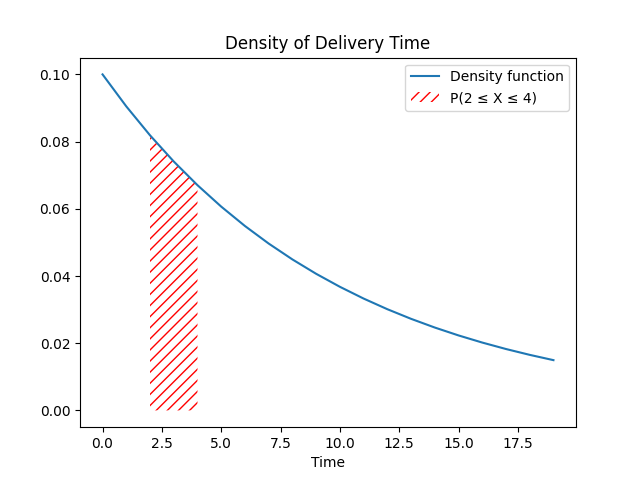
\includegraphics[width=0.7\linewidth]{figures/module_1/delivery_time_figure.png}
%    \label{fig:delivery_time_density_example}
%\end{figure}


\textbf{For continuous variables:}
\( \mathbf{P}(X = a) = 0 \)

\end{frame}
\begin{frame}{Example Discrete Random Variables}

\textbf{Business Example: Online Shop}

Let
\[
X = \text{Number of purchases per customer per month}
\]

Possible values:
\[
X \in \{0,1,2,3,\dots\}
\]


%\textbf{Definition:}

%A \textit{discrete} random variable is a function

%\[
%X : \Omega \rightarrow \mathbb{N}
%\]
%
%that assigns a numerical value to each outcome. An element $\omega \in \Omega$ is called an \textbf{observation} (here the behaviour of a customer).

\end{frame}
\begin{frame}{Example: Probability Distribution of Purchases}

\textbf{Histogram for Discrete Distribution:}

\begin{figure}
    \centering
    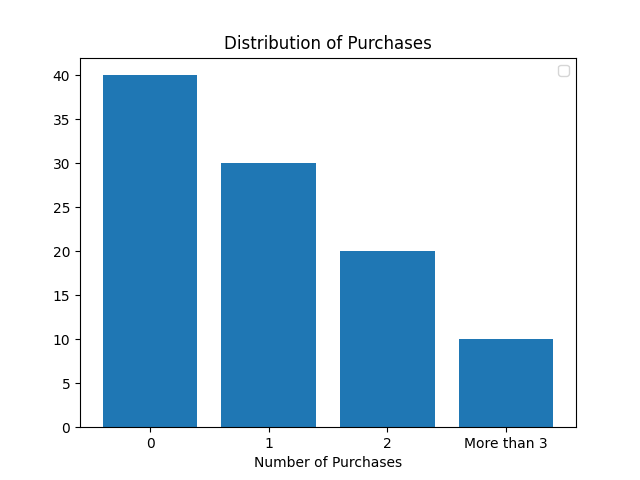
\includegraphics[width=0.8\linewidth]{figures/module_1/purchase_distribution_figure.png}
    \label{fig:purchase_distribution_example}
\end{figure}

\end{frame}

\begin{frame}{Discrete Probability Distribution}

\textbf{Business Example: Purchase Behavior}

\begin{center}
\begin{tabular}{c|c}
Purchases & Relative Frequency \\
\hline
0 & 0.4 \\
1 & 0.3 \\
2 & 0.2 \\
3+ & 0.1
\end{tabular}
\end{center}

\vspace{0.25cm}

%\textbf{Definition:}

%For a discrete random variable:

%\begin{align*}
%p(x) & = \mathbf{P}(X = x) = \mathbf{P}(\{\omega \in \Omega | X(\omega) = x\})\\
%& = \mathbf{P}(\{ \text{all customers that buy x times} \})
%\end{align*}

%with

%\[
%\sum_x p(x) = 1
%\]

\end{frame}

%\begin{frame}{Relative Frequency}
%
%\textbf{From Data to Probability}

%In practice, probabilities are often estimated from observed data.

%\medskip

%If we observe $n$ customers and $n_x$ of them buy $x$ times, the \textbf{relative frequency} is

%\[
%f(x) = \frac{n_x}{n}
%\]

%\medskip

%As the number of observations increases,
%
%\[
%f(x) \rightarrow P(X=x)
%\]

%\textbf{Idea:} Relative frequencies approximate probabilities.
%
%\end{frame}

\begin{frame}{Example: Continuous Random Variables}

\textbf{Business Example: Delivery Time}

Let

\[
X = \text{Delivery time (in days)}
\]

\textbf{Possible values:}

\[
2.13, \; 3.47, \; 4.002, \; \dots
\]

%\textbf{Definition:}

%A \textit{continuous} random variable is a function

%\[
%X : \Omega \rightarrow \mathbb{R}
%\]

%that assigns a numerical value lying in the \textit{uncountable} set of real numbers to each observation.

%\end{frame}

%\begin{frame}{Example: Probability Density of Delivery Time}

\textbf{Assumption:}
The density function of delivery time follows an exponential distribution of parameter $\lambda=0.10$ (i.e. $f(x) = \lambda \, exp(-\lambda x)$ if $x \geq 0$, else $0$).


\end{frame}
\begin{frame}

\textbf{Visualization of Probability:}

\begin{figure}
    \centering
    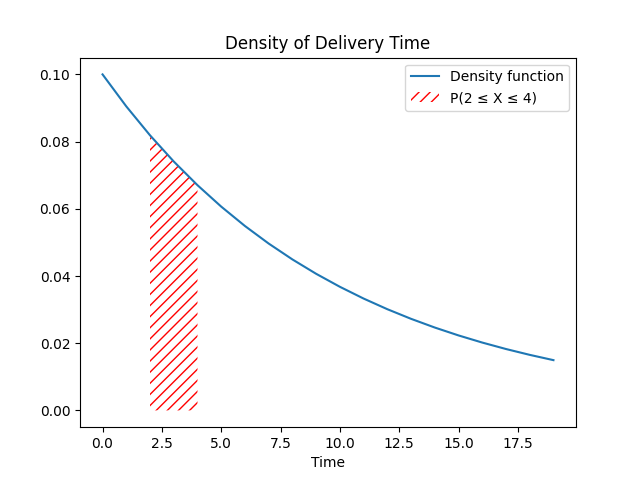
\includegraphics[width=0.7\linewidth]{figures/module_1/delivery_time_figure.png}
    \label{fig:delivery_time_density_example}
\end{figure}

\end{frame}

%\begin{frame}{Probability Density Function}
%
%\textbf{Definition:}
%A continuous random variable has a density $f(x)$ such that:
%
%\begin{itemize}
%    \item $f(x) \ge 0$
%    \item $\int_{-\infty}^{\infty} f(x)\, dx = 1$
%\end{itemize}

%\vspace{0.5cm}

%\textbf{Probability of an interval:}

%\[
%\mathbf{P}(a \le X \le b)
%=
%\int_a^b f(x)\, dx
%\]

%\vspace{0.5cm}

%\textbf{For continuous variables:}

%\[
%\mathbf{P}(X = a) = 0
%\]

%\end{frame}
\begin{frame}{From samples to distribution}
   
     Value of a random variable $\mathbf{X}$ are \textbf{samples}. 


     \medskip

     Intuitively, if $x_1,\ldots, x_t$ samples of $\mathbf{X}$, ($t$ row index),
     the the distribution can be computed:
      \[ 
        \begin{split}
		& F(a)=\hat{F}_N(a),\quad  \mbox{ for any choice $t_1 < t_2 < \ldots < t_N$, $N$ large} \\
        & \mbox{\textbf{empirical frequency}} \\
        & \hat{F}_N(a)=\frac{1}{N} (\mbox{ number of times $x_t \le a$, $t=t_1 < \ldots < t_N$})  
        \end{split}
	  \]

    \textbf{Problem} what if $x_1 < x_2 < \cdots < x_n$ ? 

    \bigskip 

    $x_1,\ldots, x_t$ should be \textbf{independently identically sampled (i.i.d) from $F$} :
 \end{frame}
 \begin{frame}{Independently sampled data}

     $x_1,\ldots, x_n$ \textbf{i.i.d} of $F$, if for any
     choice (independent of data) of non-overlapping  
     data 
     \begin{itemize}
     \item
     $z_1,\ldots, z_N$, 
     \item     
     $y_1,\ldots, y_N$ 
     \end{itemize}
     from $x_1,\ldots, x_n$ such that $N$ is large:


     \begin{itemize}
     \item \textbf{Identical probabilities:}
     \[
     \begin{split}
      &	 \frac{1}{N} (\mbox{ number of times $z_i < a$, $i=1,2,\ldots,N$}) = \\
      &	 \frac{1}{N} (\mbox{ number of times $y_i < a$, $i=1,2,\ldots,N$})=F(a)
     \end{split}
    \]
    relative frequences of events in $y_1,\ldots,y_N$, $z_1,\ldots,z_N$
    is the same. 
    \item \textbf{Independence}
    \[
     \begin{split}
      &	 \frac{1}{N} (\mbox{ number of times $z_i < a$, $y_i < b$,
           $i=1,2,\ldots,N$}) \approx F(a)F(b)
      %&	 \frac{1}{N} (\mbox{ number of times $z_i < a$, $i=1,2,\ldots,N$})
      %\\
      %&	 \times \frac{1}{N} (\mbox{ number of times $y_i < b$, $i=1,2,\ldots,N$})
     \end{split}
    \]
    \end{itemize}
    the values of $y_i$ and $z_i$ change independtly from each other. 

\end{frame}
 \begin{frame}{Independently sampled data}

    if $z_1,\ldots, z_N$ are past observations, and 
    $y_1,\ldots, y_N$ are new observations, then 
    frequencies in the past tell us about frequencies of the future. 

  %$x_t$ independently sampled from a distribution $\implies$ past observations 
%	$x_1,\ldots,\x_N$ tell us something about frequencies of new data points $x_{K}, \ldots ,x_{K+N}$, $K > N$:
 %\[
 %    \begin{split}
 %     &	 \frac{1}{N} (\mbox{ number of times $a < x_t \le b$, $t=1,\ldots, N$}) 
	% \approx 
	% \mathbf{P}(a < \mathbf{x} \le b)   \\
	%     & \approx 
	% \frac{1}{N} (\mbox{ number of times $a < x_t \le b$, $t=K,\ldots, K+N$}) 
 %   \end{split}	 
 %\]

 \bigskip

 Independence $\implies$ frequencies of  different subsets of data are the same and do not influence each other
%  \[
%    \begin{split}	  
%	  & \frac{1}{N} (\mbox{ number of times $a_1 < x_{t} \le b_1$, $a_2 < x_{K+t-1} \le b_2$, $t=1,\ldots, N$}) \approx  \\
%	  & \mathbf{P}(a_1 < \mathbf{x}_1 \le b_1, a_2 < \mathbf{x}_K \le b_2) =  \mathbf{P}(a_1 < \mathbf{x}_1 \le b_1)\mathbf{P}(a_2 < \mathbf{x}_K \le b_2) \\
%	  & \approx  \frac{1}{N} (\mbox{ number of times $a < x_t \le b$, $t=1,\ldots, N$}) \times \\
%	  & \times  \frac{1}{N} (\mbox{ number of times $a < x_t \le b$, $t=K,\ldots, K+N$}) 
%    \end{split}	  
%  \]
\end{frame}
\begin{frame}{Independent samples, independent variables}

    Two random variable $X$ and $Y$ are independent,
    \[ 
      \begin{split}
       & \mathbf{P}(X=a,Y=b)=\mathbf{P}(X=a)\mathbf{P}(Y=b), \quad 
       \mbox{discrete variable} \\
       & \mathbf{P}(X \le a,Y \le b)=\mathbf{P}(X \le a)\mathbf{P}(Y\le b), \quad 
       \mbox{continuous variable} 
      \end{split} 
    \]

   The sample $x_1,x_2,\ldots,n$ is i.i.d. sample of $F$, if
   there exists sample space $\widetilde{\Omega}$ and 
   random variables $X_1,X_2,\ldots $ on $\widetilde{\Omega}$, 
   such that 
        \begin{itemize}
        \item			
	   $x_t$ is a sample of some random variables $X_t$ 
	corresponding to the same element (row) of $\widetilde{\Omega}$,
        \item 			
		$X_t$ are \textbf{idenpendently identically distributed(i.i.d)}: have the same probability distribution $F$ and they are independent (one variable contains no information on others):

        \end{itemize}
 \medskip

	\textbf{Law of large number:} if $x_t$, $t=1,2,$ i.i.d. sample of $F$
     \[ F(a) \approx  \frac{1}{N} (\mbox{ number of times $x_t \le a$, $t=t_1 < \ldots < t_N$}) \]
%	The distribution $F$ can be reconstructed from indepent samples $x_t$, $t=1,2,\ldots$, 
%	using empirical probabilities, for large enough $N$ and any choice $t_1 < \ldots < t_N$
   %there exists a random variable $X$ whose probability distribution  is $F$, each $x_t$ is a sample of $\mathbf{x}$, and 
   %for large enough $N$: 
	

\end{frame}






\begin{frame}{Expected value of a random variable}

 Expected value of $\mathbf{E}[X]$:


 \begin{itemize}
 \item $X$ takes discrete values:
    $$\mathbf{E}[X]=\sum_{i=1}^{\infty} i \mathbf{P}(X=i)$$


 \medskip

 \item $X$ has continuous values:

    \[ \mathbf{E}[X]=\int_{-\infty}^{+\infty} x f(x)dx \]
 \end{itemize}



  \begin{center}

  $m_{X}=\mathbf{E}[X]$ -- mean of $X$.

  \end{center}

  \medskip
  $(X-m_{X})^2$ is a random variable: 

  \begin{center}


      $\sigma_{X}=\sqrt{\mathbf{E}[(X-m_{X})^2]}$ standard deviation,

      $\sigma_{X}^2$ -- variance of $X$.
  
  \end{center}

  Example:Gaussian  distribution: $f(x)=\frac{1}{\sigma \sqrt{2\pi}} e^{-\frac{(x-m)^2}{2\sigma^2}}$,  
      mean $m$,variance $\sigma^2$.

\end{frame}
\begin{frame}{Expected value of a random variable}

 Expectation, variance depend on the distribution $F$ of $X$. 

 \medskip

 $x_t$ independently, randomly sampled from $F$:

    \[ m_{X}=\mathbf{E}[X]  \approx \bar{x}=\frac{1}{N} \sum_{t=1}^{N} x_t \]
      \[ \sigma_{X}^2=\mathbf{E}[(X-m_{X})^2] \approx  \frac{1}{N-1} \sum_{t=1}^{N} (x_t - \bar{x})^2 \]

  \medskip

  

  Interpretation of standard deviation:


 \[ \mathbf{P}(|X - m_{X}| > a) \le \frac{\sigma_{X}^2}{a^2} \]


   The smaller the standard deviation is, the more the points $x_t$ are concentrated around the mean.


\end{frame}
\begin{frame}{Covariance, correlation and independence}
\textbf{Covariance:}

The covariance of two random variables $X$ and $Y$ is:

\[
\mathrm{Cov}(X, Y) = \mathbb{E}[(X - \mathbb{E}[X])(Y - \mathbb{E}[Y])]
\]

\vspace{0.3cm}

Measures how much $X$ and $Y$ vary together.

\vspace{0.5cm}

\textbf{Correlation:}

The correlation coefficient is:

\[
\rho(X, Y) = \frac{\mathrm{Cov}(X, Y)}{\sigma_X \sigma_Y}
\]

\vspace{0.3cm}

Normalized to $[-1, 1]$:
\begin{itemize}
    \item $\rho = 1$ → perfect positive correlation
    \item $\rho = 0$ → no linear relationship
    \item $\rho = -1$ → perfect negative correlation
\end{itemize}

\vspace{0.5cm}

\textbf{Independence and Covariance:}

If $X$ and $Y$ are independent, then:

\[
\mathrm{Cov}(X, Y) = 0
\]

Conversely, zero covariance does not necessarily imply independence.
\end{frame}
\begin{frame}{Mean, variance from data, visualization}

 \lstinline$np.mean(X)$, \lstinline$np.std(X)$, \lstinline$np.var(X)$.

 \medskip

    Historgrams are concentrated around the mean, they get flatter with the increase of standard deviation (more points far away from the mean).

 \begin{center}	
    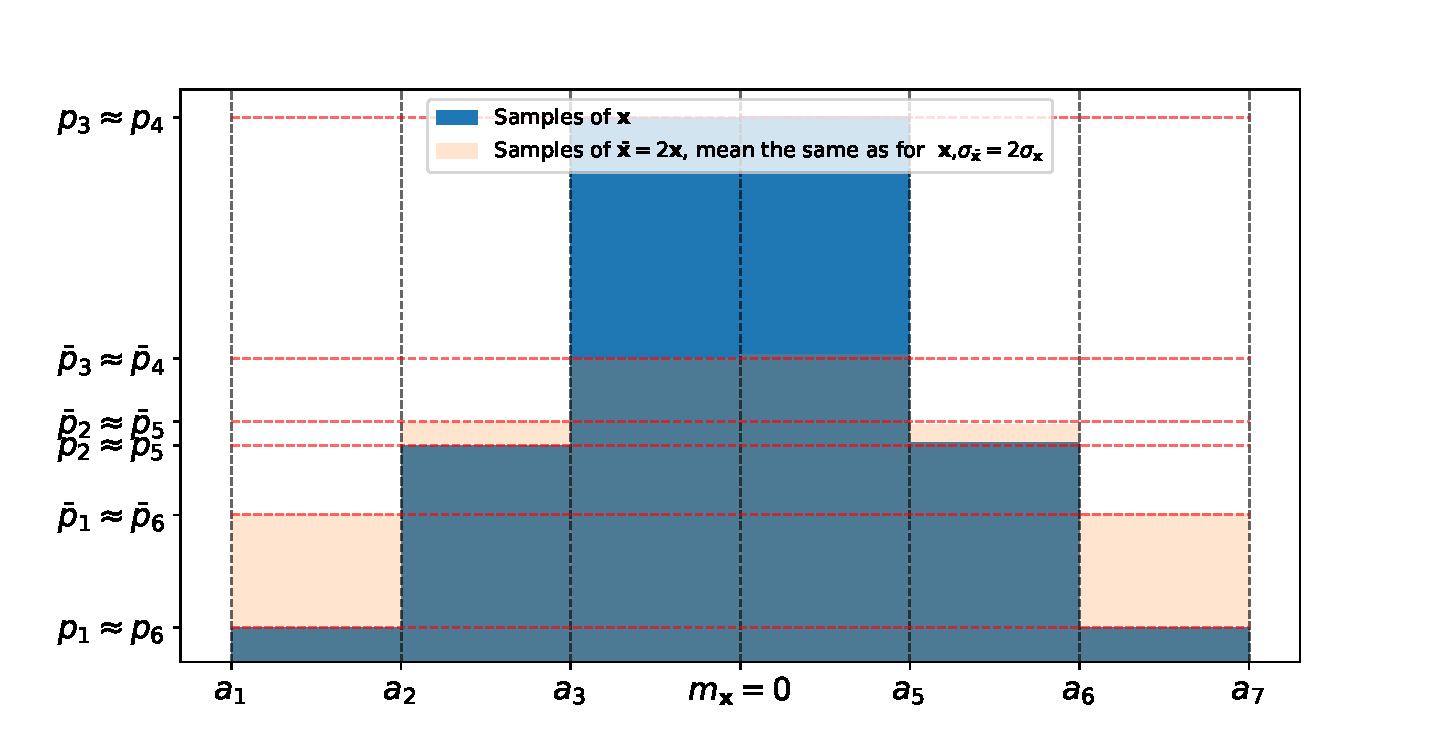
\includegraphics[scale=0.4]{Figure_6V.pdf}
  \end{center}

\end{frame}

\begin{frame}{Example: Expectation of Discrete Probability Distribution}
 \textbf{Assumption:}
The density function of delivery time follows an exponential distribution of parameter $\lambda=0.10$ (i.e. $f(x) = \lambda \, exp(-\lambda x)$ if $x \geq 0$, else $0$).


\textbf{Business Example: Average Purchases}

\[
\mathbb{E}[X] = \sum_x x \cdot \mathbf{P}(X=x)
\]

\[
= 0(0.4) + 1(0.3) + 2(0.2) + 3(0.1) = 0.7
\]

\vspace{0.5cm}

\textbf{Interpretation:}

\begin{itemize}
    \item The purchase average is nearly $1$
    \item It is possible to estimate the expected revenue 
\end{itemize}

\end{frame}

\begin{frame}{Example: Expectation of Probability Density Function}


\[
\mathbb{E}[X] = \int_{-\infty}^{+\infty} x \, f(x) \, dx = \frac{1}{\lambda} = 10
\]

\vspace{0.5cm}

\textbf{Business Interpretation:}

\begin{itemize}
    \item The average of delivery time is $10$ days
    \item It is possible to estimate the delivery delay between two customers.
\end{itemize}

\end{frame}

\begin{frame}{Variance and Risk}

\textbf{Business Question:}

Two segments have the same average revenue. Which one is riskier?

\vspace{0.5cm}

\[
\mathrm{Var}(X) = \mathbb{E}[(X - \mathbb{E}[X])^2]
\]

\vspace{0.5cm}

Variance measures variability and business risk. 

\end{frame}

\begin{frame}{Normal Distribution}

\textbf{Definition:}

A random variable $X$ follows a normal distribution if its density is:

\[
f(x) =
\frac{1}{\sqrt{2\pi \sigma^2}}
\exp\left(
-\frac{(x-\mu)^2}{2\sigma^2}
\right)
\]

\vspace{0.5cm}

Notation:

\[
X \sim \mathcal{N}(\mu, \sigma^2)
\]

\textbf{Properties:}

\begin{itemize}
    \item $\mathbb{E}(X) = \mu$: mean
    \item $\mathrm{Var}(X) = \sigma^2$: variance
\end{itemize}

\end{frame}

\begin{frame}{Normal Distribution Density}

\textbf{Illustration:}

\begin{figure}
    \centering
    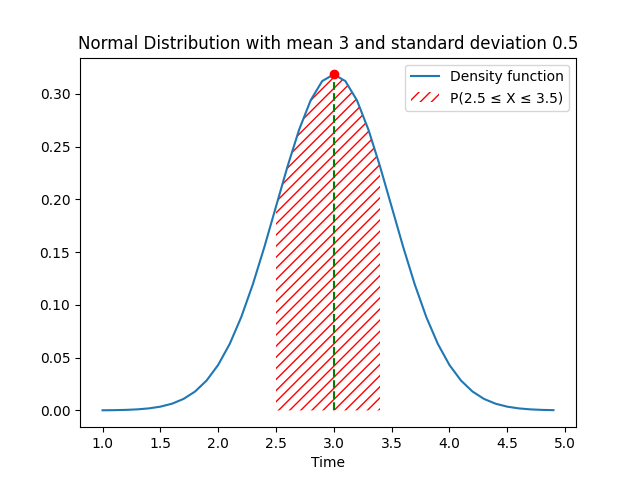
\includegraphics[width=0.8\linewidth]{figures/module_1/normal_distribution_figure.png}
    \label{fig:normal_distribution_example}
\end{figure}
    
\end{frame}

\begin{frame}{Example: Normal Delivery Time}

Assume delivery time follows:

\[
X \sim \mathcal{N}(3, 0.5^2)
\]

\vspace{0.5cm}

\begin{itemize}
    \item Mean = 3 days
    \item Standard deviation = 0.5 days
\end{itemize}

\vspace{0.5cm}

We can compute:

\[
\mathbf{P}(2.5 \le X \le 3.5)
\]

\end{frame}

\begin{frame}{Interpretation of Parameters}

\textbf{Mean $\mu$:}
\begin{itemize}
    \item Determines the center
    \item Shifts the distribution
\end{itemize}

\vspace{0.3cm}

\textbf{Variance $\sigma^2$:}
\begin{itemize}
    \item Controls spread
    \item Larger variance $\Rightarrow$ flatter curve
    \item Smaller variance $\Rightarrow$ more concentrated
\end{itemize}

\vspace{0.5cm}

The normal distribution is symmetric around $\mu$.

\end{frame}

\begin{frame}{The 68--95--99.7 Rule}

\textbf{Empirical Rule for the Normal Distribution}

If

\[
X \sim \mathcal{N}(\mu, \sigma^2)
\]

then approximately:

\[
\mathbf{P}(|X - \mu| \le \sigma) \approx 68\%
\]

\[
\mathbf{P}(|X - \mu| \le 2\sigma) \approx 95\%
\]

\[
\mathbf{P}(|X - \mu| \le 3\sigma) \approx 99.7\%
\]

\vspace{0.5cm}

\textbf{Business Interpretation:}

Standard deviation directly quantifies risk and uncertainty.

\end{frame}

%%\begin{frame}{Conditional Probability}
%%
%%\textbf{Business Example: Online Advertising}
%%
%%\[
%%\mathbf{P}(\text{Buy} \mid \text{Click})
%%\]
%%
%%\vspace{0.5cm}
%%
%%\textbf{Definition:}
%%
%%\[
%%\mathbf{P}(A \mid B) = \frac{\mathbf{P}A \cap B)}{\mathbf{P}(B)}
%%\]
%%
%%\vspace{0.5cm}
%%
%%Conditional probability models dependence between events.
%%
%%\end{frame}
%%
%%\begin{frame}{Fraud Detection Example}
%%
%%\textbf{Insurance Fraud}
%%
%%\begin{itemize}
%%    \item 2\% of claims are fraudulent
%%    \item 90\% of fraudulent claims are flagged
%%    \item 5\% of legitimate claims are falsely flagged
%%\end{itemize}
%%
%%\vspace{0.5cm}
%%
%%Question:
%%
%%\begin{center}
%%If a claim is flagged, what is the probability it is truly fraudulent?
%%\end{center}
%%
%%\end{frame}
%%
%%\begin{frame}{Bayes' Theorem}
%%
%%\[
%%\mathbf{P}(A \mid B) = \frac{\mathbf{P}(B \mid A) \mathbf{P}(A)}{\mathbf{P}(B)} = \frac{\mathbf{P}(B \mid A) \mathbf{P}(A)}{\mathbf{P}(B | A) \mathbf{P}(A) + \mathbf{P}(B | \overline{A}) \mathbf{P}(\overline{A})}
%%\]
%%
%%\vspace{0.5cm}
%%
%%\textbf{Interpretation:}
%%
%%\begin{itemize}
%%    \item $\mathbf{P}(A)$: Prior belief
%%    \item $\mathbf{P}(B \mid A)$: Likelihood
%%    \item $\mathbf{P}(A \mid B)$: Posterior belief
%%\end{itemize}
%%
%%\vspace{0.5cm}
%%
%%Bayes' theorem updates beliefs using new evidence.
%%
%%\end{frame}
%%
%%\begin{frame}{Bayesian Update in Fraud Detection}
%%
%%\[
%%\mathbf{P}(F \mid \text{Flag}) =
%%\frac{0.9 \cdot 0.02}
%%{0.9 \cdot 0.02 + 0.05 \cdot 0.98}
%%\]
%%
%%\vspace{0.5cm}
%%
%%Result:
%%
%%\[
%%\mathbf{P}(F \mid \text{Flag}) \approx 27\%
%%\]
%%
%%\vspace{0.5cm}
%%
%%Even highly accurate systems can produce many false alarms
%%when the base rate is small.
%%
%%\end{frame}
%%
%%\begin{frame}{A/B Testing Example}
%%
%%\textbf{New Checkout Design}
%%
%%\begin{itemize}
%%    \item After 20 users: conversion = 70\%
%%    \pause
%%    \item After 20,000 users: conversion = 12\%
%%\end{itemize}
%%
%%\pause
%%
%%\vspace{0.5cm}
%%
%%Why does the estimate change so much?
%%
%%\end{frame}

\begin{frame}{Business Meaning of LLN}

The Law of Large Numbers explains:

\begin{itemize}
    \item Why large datasets reduce noise
    \item Why small samples are unreliable
    \item Why ML improves with more data
\end{itemize}

\vspace{0.5cm}

Large data stabilizes estimates. This comes from the following inequality which holds for all $\epsilon > 0$:

\[ \mathbf{P}(|\bar{X}_n - \mu| > \epsilon) \le \frac{V(\bar{X}_n)}{\epsilon^2} \]

\end{frame}

\begin{frame}{Why Does the Average Look Normal?}

\textbf{Customer Spending Example}

Individual spending is highly skewed.

\vspace{0.3cm}

\pause

However:

\begin{itemize}
    \item The average of 500 customers
    \item Appears approximately normal
\end{itemize}

\vspace{0.5cm}

Why?

\end{frame}

\begin{frame}{Central Limit Theorem}

Let $X_1, \dots, X_n$ be i.i.d. with

\[
\mathbb{E}[X_i] = \mu, 
\quad
\mathrm{Var}(X_i) = \sigma^2
\]

Then:

\[
\frac{\bar{X}_n - \mu}{\sigma / \sqrt{n}}
\rightarrow \mathcal{N}(0,1)
\]

as $n \to \infty$.

\end{frame}

\begin{frame}{Business Meaning of the CLT}

For large $n$:

\[
\bar{X}_n \approx \mathcal{N}
\left(
\mu, \frac{\sigma^2}{n}
\right)
\]

\vspace{0.5cm}

Implications:

\begin{itemize}
    \item Enables confidence intervals
    \item Enables A/B testing
    \item Uncertainty decreases with $\sqrt{n}$
\end{itemize}

\end{frame}

\begin{frame}{Market Research Example}

A survey of 1000 customers:

\begin{itemize}
    \item 180 would buy the product
\end{itemize}

\vspace{0.5cm}

Estimated probability:

\[
\hat{p} = 0.18
\]

\vspace{0.5cm}

Is this the true purchase probability?

\end{frame}

\begin{frame}{Population vs Sample}

\textbf{Population parameter:}

\[
p = \text{True purchase probability}
\]

\vspace{0.5cm}

\textbf{Sample estimate:}

\[
\hat{p} = \frac{\text{Number of buyers}}{n}
\]

\vspace{0.25cm}

In practice, we only observe samples.

\end{frame}

\begin{frame}{Confidence Interval}

Using the CLT:

\[
\bar{X} \pm 1.96 \frac{\sigma}{\sqrt{n}}
\]

\vspace{0.25cm}

\textbf{Interpretation}:

If we repeated the study many times,
95\% of the intervals would contain the true parameter.

\end{frame}


\begin{frame}[fragile]{Exercise: Histogram with Relative Frequency}

\begin{itemize}
    \item Is the wage distribution symmetric, left-skewed, or right-skewed?
    \item Where are most wages concentrated?
    \item Are there extreme values or outliers?
\end{itemize}
    
\end{frame}

\begin{frame}[fragile]{Exercise: Histogram with Relative Frequency}

\begin{minted}{python}
import pandas as pd
import matplotlib.pyplot as plt

# Load data
df = pd.read_csv("Wage_merged.csv")

wages = df["wage"]

# Histogram with relative frequency
plt.hist(wages, bins=20, density=True)

plt.xlabel("Hourly Wage")
plt.ylabel("Relative Frequency")
plt.title("Distribution of Hourly Wages")

plt.show()
\end{minted}
    
\end{frame}

\begin{frame}[fragile]{Exercise: Law of Large Numbers (LLN)}

\begin{itemize}
    \item What happens to the sample mean when the sample size increases?
    \item What happens to the variance of the estimator as the sample size grows?
    \item Are there extreme values or outliers?
\end{itemize}
    
\end{frame}

\begin{frame}[fragile]{Exercise: Law of Large Numbers (LLN)}

\begin{minted}{python}
import numpy as np

wages = df["wage"]
true_mean = wages.mean()

sample_sizes = range(5, 500)
means = []

for n in sample_sizes:
    sample = wages.sample(n, replace=True)
    means.append(sample.mean())

plt.plot(sample_sizes, means, label="Sample Mean")
plt.axhline(true_mean, linestyle="--", label="True Mean")

plt.xlabel("Sample Size")
plt.ylabel("Mean Wage")
plt.title("Law of Large Numbers")

plt.legend()
plt.show()
\end{minted}
    
\end{frame}

\begin{frame}[fragile]{Exercise: Central Limit Theorem (CLT)}

\begin{itemize}
    \item Is the sample means distribution symmetric, left-skewed, or right-skewed?
    \item What happens if we increase the sample size from 30 to 100?
\end{itemize}
    
\end{frame}

\begin{frame}[fragile]{Exercise: Central Limit Theorem (CLT)}

\begin{minted}{python}
sample_size = 30
num_samples = 1000

sample_means = []

for _ in range(num_samples):
    sample = wages.sample(sample_size, replace=True)
    sample_means.append(sample.mean())

plt.hist(sample_means, bins=30, density=True)

plt.xlabel("Sample Mean Wage")
plt.ylabel("Density")
plt.title("Central Limit Theorem")

plt.show()
\end{minted}
    
\end{frame}
\begin{frame}{Machine learning}

 Black box process
\begin{figure}
\begin{center}
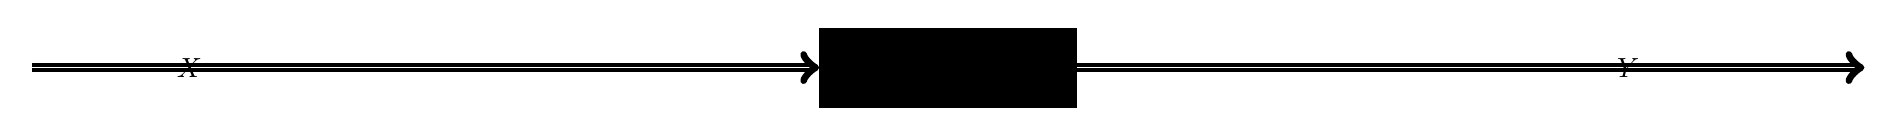
\begin{tikzpicture}
 \tikzstyle{mode}=[draw,transform shape, minimum size=10mm]
 \node[draw,right, fill=black, text centered, text width=20ex,transform shape, minimum size = 10mm] at 
    (0,0) (SW) {}; % \textbf{Black box}};
 \draw[very thick, double,->] (SW.east)++(0,0) -- ++(10,0) node[pos=0.7]{$Y$};
 \draw[very thick, double,<-] (SW.west)++(0,0) -- ++(-10,0) node[pos=0.8]{$X$};
\end{tikzpicture}
\end{center}
\end{figure}

\medskip

$X,Y$ random variables.


  \medskip


  Find a function $f$ such that

  \begin{figure}
\begin{center}
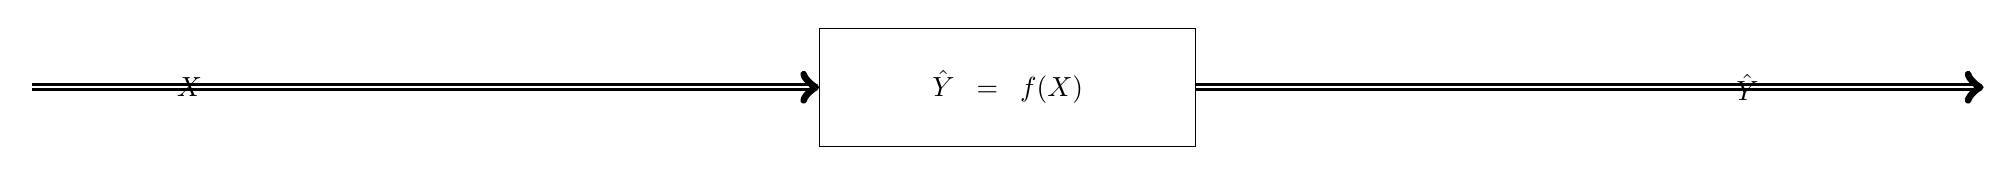
\begin{tikzpicture}
 \tikzstyle{mode}=[draw,transform shape, minimum size=10mm]
  \node[draw,right, text centered, text width=30ex,transform shape, minimum size = 15mm] at 
  (0,0) (SW) 
  { $\hat{Y}=f(X)$ };
  \draw[very thick, double,->] (SW.east)++(0,0) -- ++(10,0) node[pos=0.7]{$\hat{Y}$};
  \draw[very thick, double,<-] (SW.west)++(0,0) -- ++(-10,0) node[pos=0.8]{$X$};
\end{tikzpicture}
\end{center}
\end{figure}


and the probability of $(Y-\hat{Y})$ being large is not too big, i.e, \textcolor{blue}{expected prediction error (true loss)}
\[ 
  \mathbf{E}[(Y-\hat{Y})^2] \mbox{ or more generally }
  \mathbf{E}[\ell(Y,\hat{Y})]
\]

is small,  $\ell(y,y')$ a measure of how close $y$ and $y'$ are.? 

\medskip

\end{frame}
\begin{frame}{Machine learning}
 

	We do not fully know the distribution of $X,Y$.

\medskip

	$E[\ell(Y, \hat{Y})]$, $\hat{Y}=f(X)$  -- depends on the distribution of $X,Y$


 \bigskip

	We know i.i.d. samples $x_1,\ldots, x_N$ of $X$
    and $y_1,\ldots,y_N$ of $Y$, $x_i,y_i$ correspond to the same row (outcome)

  \bigskip

  Basic soluton: find $f$ for which: 
   \[ \frac{1}{N} \sum_{i=1}^{N} \ell(y_i,f(x_i))+ \mbox{some cleverly chosen term} \]

   is small. 


  \medskip

   Question:  will 
           $$E[(\ell(Y,f(X))]$$

   be small, if  
   \( \frac{1}{N} \sum_{i=1}^{N} \ell(y_i,f(x_i))+ \mbox{some cleverly chosen term} \)

    is small ? 
    

\end{frame}
\begin{frame}{Tearser for future: generalisation bounds}
  If $x_1,x_2,\ldots, x_N$ i.i.d. sample
of $F$, then with probability at least $1-\delta$:

\[
\underbrace{\mathbb{E}[\ell(Y, f(X))]}_{\text{true loss}} \le \underbrace{\frac{1}{N} \sum_{i=1}^{N} \ell(y_i, f(x_i))}_{\text{empirical loss}} + \frac{C}{\sqrt{N}} \sqrt{\log(1/\delta)}
\]

where $C$ depends on the complexity of the model class $\mathcal{F}$, measured by:

\begin{itemize}
    \item \textbf{VC dimension:} Growth rate of different models which behave the same way on finite samples
    \item \textbf{Rademacher complexity:} Average correlation with random labels
\end{itemize}

\medskip 

\begin{itemize}
    \item Higher model complexity $\Rightarrow$ Larger $C$
    \item Larger sample size $N$ $\Rightarrow$ Tighter bound (decreases as $1/\sqrt{N}$)
    \item The bound trades off: training error vs model complexity
    \item Smaller $\delta$ (higher confidence) $\Rightarrow$ Larger bound (looser guarantee)
\end{itemize}

\end{frame}
\begin{frame}{Learning from Data: Estimating Distributions}

\textbf{Key Insight:}

Estimating the mean, variance, and distribution from data is itself a form of machine learning.

\textbf{Given i.i.d. samples:}
\(
x_1, x_2, \ldots, x_N 
\) from $F$.

We estimate the population parameters:


\textbf{Empirical Mean:}

\[
\hat{m} = \frac{1}{N} \sum_{i=1}^{N} x_i \quad \text{estimates} \quad \mu = \mathbb{E}[X]
\]

\textbf{Empirical Distribution:}

\[
\hat{F}(a) = \frac{1}{N} \#\{i : x_i \le a\} \quad \text{estimates} \quad F(a) = \mathbb{P}(X \le a)
\]


These are \textbf{learned models} from data, just like any other ML model.

\end{frame}
\section{Hypothesis testing}
\begin{frame}{Why hypothesis testing}
\textbf{Problem:} Different datasets yield different model estimates.

\vspace{0.5cm}

\textbf{Example:}
\begin{itemize}
    \item Dataset 1: Sample mean $\hat{m}_1 = 10.2$
    \item Dataset 2: Sample mean $\hat{m}_2 = 10.5$
    \item True population mean: unknown
\end{itemize}

\vspace{0.5cm}

\textbf{Question:} Is the difference real or just noise?

\vspace{0.5cm}

Hypothesis testing provides a framework to assess whether observed differences are statistically significant or due to random sampling variation.

\vspace{0.5cm}

\textbf{Key Models We Estimate from Data:}
\begin{itemize}
    \item Empirical mean: $\hat{m} = \frac{1}{N}\sum x_i$
    \item Empirical variance: $\hat{\sigma}^2 = \frac{1}{N-1}\sum (x_i - \hat{m})^2$
    \item Empirical distribution: $\hat{F}(a) = \frac{\text{count}(x_i \le a)}{N}$
\end{itemize}

\vspace{0.5cm}

All depend on random samples, so they fluctuate. Hypothesis testing quantifies this uncertainty.

\end{frame}
%%\begin{frame}{Notions from statistics}
%%    A statistic $\mathbf{T}$ is a function of an i.i.d. sample $x_1, \ldots, x_N$ that serves to estimate a parameter of the probability distribution.
%%
%%    \medskip
%%
%%    The statistic $\mathbf{T}$ depends on the observed data $x_1, \ldots, x_N$, so its value changes whenever we collect a new sample.
%%
%%    \medskip
%%
%%     Examples:
%%     
%%    \[ \hat{m} = \frac{1}{N} \sum_{t=1}^{N} x_t \]
%%     estimates the mean,
%%
%%    \[ \hat{\sigma}^2 = \frac{1}{N-1} \sum_{t=1}^{N} (x_t - \hat{m})^2 \]
%%
%%     estimates the variance,
%%
%%    \[ \hat{F}(x) = \frac{1}{N} \mbox{ number of times } x_i \le x \]
%%
%%    estimates the probability distribution. 
%%
%%    \medskip
%%
%%    We want a statistic $\mathbf{T}$ to be:
%%
%%    \begin{itemize}
%%    \item \textbf{Unbiased:} $\mathbb{E}[\mathbf{T}] = \theta_*$ (true parameter). 
%%    
%%                 The \textbf{bias} is $\theta_* - \mathbb{E}[\mathbf{T}]$.
%%
%%    \item \textbf{Consistent:} $\mathbf{T}$ converges to the true value as $N \to \infty$.
%%
%%    \item \textbf{Efficient:} $\mathbf{T}$ has small variance that decreases to zero as $N$ grows.
%%    \end{itemize}
%%
%%\end{frame}

\begin{frame}{Hypothesis Testing for the Mean}

\textbf{Setup:} We observe i.i.d. samples $x_1, \ldots, x_N$ and want to test if the true mean is $\mu_0$.

\vspace{0.3cm}

\textbf{Null hypothesis:} $H_0: \mu = \mu_0$

\textbf{Alternative hypothesis:} $H_1: \mu \ne \mu_0$

\vspace{0.5cm}

\textbf{Test statistic:}

\[
t = \frac{\hat{m} - \mu_0}{\hat{\sigma}}
\]

where $\hat{m} = \frac{1}{N}\sum x_i$ and $\hat{\sigma} = \sqrt{\frac{1}{N-1}\sum(x_i - \hat{m})^2}$.

\vspace{0.3cm}

\textbf{Key fact (Central Limit Theorem):}

Under $H_0$, the test statistic $t$ approximately follows a Student's t-distribution (roughly normal for large $N$).

\end{frame}

\begin{frame}{Decision Rule}

We choose a significance level $\alpha$ (typically 0.05).

\vspace{0.3cm}

\textbf{Critical value:} Find $c$ such that $\mathbb{P}(|t| > c) = \alpha$, if $\mu_0$ is the true mean.

\vspace{0.3cm}

\textbf{Rejection rule:} Reject $H_0$ if $|t| > c$.

\vspace{0.5cm}

\textbf{Interpretation:}

If $H_0$ were true, observing $|t| > c$ would be very unlikely (probability $\alpha$).  
Since we observed it, we reject $H_0$.

\vspace{0.3cm}

\textbf{p-value:} The smallest $\alpha$ for which we reject $H_0$.  
If p-value $< 0.05$, reject $H_0$.

\end{frame}

\begin{frame}{Example: Mean Wage Test}

\textbf{Observed data:} $\hat{m} = 10.5$, $\hat{\sigma} = 0.2$, $N = 100$

\medskip

\textbf{Test:} Is the true mean wage equal to 10?

\medskip

\textbf{Test statistic:}
\[ t = \frac{10.5 - 10}{0.2} = 2.5 \]

\medskip

\textbf{Critical value at $\alpha = 0.05$:} $c \approx 1.98$

\medskip

\textbf{Decision:} Since $|t| = 2.5 > 1.98$, we reject $H_0$.

\medskip

\textbf{Conclusion:} The true mean wage is significantly different from 10 dollars.

\end{frame}

\begin{frame}{Confidence Intervals}

From the test statistic, we can construct a confidence interval.

\vspace{0.3cm}

Choose $c$ such that $\mathbb{P}(|t| \le c) = 1 - \alpha$.

\vspace{0.3cm}

Then with probability $1-\alpha$:

\[
\hat{m} - c \cdot \hat{\sigma} \le \mu \le \hat{m} + c \cdot \hat{\sigma}
\]

\vspace{0.3cm}

\textbf{Interpretation:}

The confidence interval contains all values $\mu_0$ for which we cannot reject $H_0: \mu = \mu_0$ at significance level $\alpha$.

\vspace{0.3cm}

\textbf{Example:} If the 95\% confidence interval is $[10.1, 10.9]$, we can reject $H_0: \mu = 10$ but not $H_0: \mu = 10.5$.

\end{frame}

\begin{frame}{Two-Sample Hypothesis Testing}

\textbf{Problem:} Compare means of two independent groups.

\vspace{0.3cm}

\textbf{Data:}
\begin{itemize}
    \item Group 1: $x_1, \ldots, x_N$ with mean $\hat{m}_1$ and variance $\hat{\sigma}_1^2$
    \item Group 2: $y_1, \ldots, y_M$ with mean $\hat{m}_2$ and variance $\hat{\sigma}_2^2$
\end{itemize}

\vspace{0.3cm}

\textbf{Hypotheses:}

$H_0: \mu_1 = \mu_2$ (means are equal)

$H_1: \mu_1 \ne \mu_2$ (means differ)

\end{frame}

\begin{frame}{Two-Sample t-Test}

\textbf{Test statistic:}

\[
t = \frac{\hat{m}_1 - \hat{m}_2}{\sqrt{\frac{\hat{\sigma}_1^2}{N} + \frac{\hat{\sigma}_2^2}{M}}}
\]

\vspace{0.3cm}

Under $H_0$, $t$ approximately follows a t-distribution (by CLT).

\vspace{0.3cm}

\textbf{Decision:} Reject $H_0$ if $|t| > c$ (critical value at significance level $\alpha$).

\vspace{0.3cm}

\textbf{Business Example:}

Compare average wages between men and women.  
If $|t|$ is large, evidence suggests systematic wage differences.

\end{frame}

\begin{frame}{Example: Mean wage of 10 dollars}

\textbf{Observed data:} $\hat{m} = 10.5$, $\hat{\sigma} = 0.2$, $N = 100$

\medskip

\textbf{Test statistic:}
\[ t = \frac{10.5 - 10}{0.2} = \frac{0.5}{0.2} = 2.5 \]

\medskip

\textbf{Critical value at $\alpha = 0.05$:} $c \approx 1.98$ (from t-distribution with 99 degrees of freedom)

\medskip

\textbf{Decision:} Since $|t| = 2.5 > 1.98$, we reject $H_0$.

\medskip

\textbf{Conclusion:} The evidence strongly suggests that the true mean wage is not 10 dollars; it is likely higher.

\end{frame}

\begin{frame}{Examples}

         \textbf{Example (t-test):} Let $x_1, \ldots, x_N$ be an i.i.d. sample with unknown mean $\mu$ and variance $\sigma^2$. 
         
         The null hypothesis is $H_0: \mu = 0$. 

        \[\mathbf{T} = \hat{m} = \frac{1}{N} \sum_{i=1}^{N} x_i\]

        \[\hat{\sigma} = \sqrt{\frac{1}{N(N-1)} \sum_{i=1}^{N} (x_i - \hat{m})^2}\]

         The test statistic 
         \[\frac{\mathbf{T}}{\hat{\sigma}}\]
         follows a Student's t-distribution. For large $N$, it is approximately normal.

        \medskip	
         
            Other examples include the Kolmogorov-Smirnov test, Bernoulli test, etc. 	   
     
            \medskip

             Python: \lstinline$scipy.stats.ttest_1samp$, \lstinline$scipy.stats.ks_1samp$, \lstinline$scipy.stats.binomtest$.

\end{frame}

\begin{frame}{Extensions of hypothesis testing}

        \textbf{Non-zero null hypothesis:} $H_0: \theta = \theta_0$

        \medskip

         \textbf{One-sided alternative:} Instead of $H_1: \theta \ne \theta_0$, use $H_1: \theta > \theta_0$ or $H_1: \theta < \theta_0$.
         
         We reject $H_0$ if $\mathbf{T} > c$ or $\mathbf{T} < c$ (respectively) instead of $|\mathbf{T}| > c$.

     \medskip
         
         \textbf{Two-sample hypothesis test:} 
         \begin{itemize}
                     \item Let $x_1, \ldots, x_N$ be an i.i.d. sample with parameter $\theta_1$.
                     \item Let $y_1, \ldots, y_M$ be an i.i.d. sample with parameter $\theta_2$.
                     \item $H_0: \theta_1 = \theta_2$, $H_1: \theta_1 \ne \theta_2$.
                    \end{itemize}			   

         We reject $H_0$ if $|\mathbf{T}| > c$, where the distribution of $\mathbf{T}$ under $H_0$ is known.

         Examples: Kolmogorov-Smirnov test, t-test, Spearman's correlation, Pearson's correlation.
                     
         Python: \lstinline$scipy.stats.ttest_2samp$, \lstinline$scipy.stats.ks_2samp$, \lstinline$scipy.stats.spearmanr$.

\end{frame}	   

\begin{frame}{Confidence intervals}
         
         Choose $c$ such that 

        \[ \left|\frac{\mathbf{T} - \theta}{\hat{\sigma}}\right| > c \]
         
        with probability $\alpha$.

        Then with probability $1-\alpha$:

        \[ 
    \begin{split}
                \mathbf{T} - c \hat{\sigma} \le \theta \le \mathbf{T} + c \hat{\sigma}
             \end{split}
        \]

\end{frame}

\begin{frame}{Confidence intervals}

     The probability of observing data such that $\theta$ falls outside the interval

     \[   
             [\mathbf{T} - c \hat{\sigma}, \mathbf{T} + c \hat{\sigma}]
    \]

     is $\alpha$.

    \medskip

     This interval is the \textbf{confidence interval} at significance level $\alpha$ (or confidence level $1-\alpha$).

    \medskip

    Typically $\alpha = 0.02$ or $\alpha = 0.05$.

    \medskip

     For any $\theta_*$ in the confidence interval, we cannot reject the null hypothesis $H_0: \theta = \theta_*$ at significance level $\alpha$.

    \medskip

     If the confidence interval contains $0$, we cannot reject that $\theta = 0$. 

\end{frame}
\begin{frame}[fragile]{Exercise: Confidence Interval for the Mean Wage}

\begin{itemize}
    \item If we collect new wages different from the dataset, what would be the range of values with 95\% of confidence ?
\end{itemize}
    
\end{frame}

\begin{frame}[fragile]{Exercise: Confidence Interval for the Mean Wage}

\begin{minted}{python}
wages = df["wage"]

n = len(wages)
mean_wage = wages.mean()
std_wage = wages.std(ddof=1)

# Standard error
se = std_wage / np.sqrt(n)

# 95% confidence interval
ci = stats.t.interval(0.95, df=n-1, loc=mean_wage, scale=se)

print("Mean wage:", mean_wage)
print("95% confidence interval:", ci)
\end{minted}
    
\end{frame}

\begin{frame}[fragile]{Exercise: One-Sample Hypothesis Test}

\begin{itemize}
    \item If we collect new wages different from the dataset, what would be the range of values with 95\% of confidence ?
\end{itemize}
    
\end{frame}

\begin{frame}[fragile]{Exercise: One-Sample Hypothesis Test}

\begin{minted}{python}
from scipy.stats import ttest_1samp

t_stat, p_value = ttest_1samp(wages, 10)

print("t-statistic:", t_stat)
print("p-value:", p_value)
\end{minted}

\end{frame}
\begin{frame}[fragile]{Exercise: Two-Sample Hypothesis Test}

\begin{itemize}
    \item Are wages significantly different between men and women?
    \item What is the null hypothesis?
    \item What does the p-value tell us?
\end{itemize}
    
\end{frame}
%\begin{frame}{Two-Sample t-Test: Test Statistic}

%\textbf{Setup:} We observe two independent i.i.d. samples:
%\begin{itemize}
%    \item Sample 1: $x_1, \ldots, x_N$ with mean $\hat{m}_1$ and variance $\hat{\sigma}_1^2$
%    \item Sample 2: $y_1, \ldots, y_M$ with mean $\hat{m}_2$ and variance $\hat{\sigma}_2^2$
%\end{itemize}

%\vspace{0.3cm}

%\textbf{Null hypothesis:} $H_0: \mu_1 = \mu_2$

%\textbf{Alternative hypothesis:} $H_1: \mu_1 \ne \mu_2$
%
%\vspace{0.5cm}

%\textbf{Test statistic:}

%\[
%t = \frac{\hat{m}_1 - \hat{m}_2}{\sqrt{\frac{\hat{\sigma}_1^2}{N} + \frac{\hat{\sigma}_2^2}{M}}}
%\]

%\vspace{0.3cm}

%\textbf{Key fact (Central Limit Theorem):}

%Under $H_0$, the test statistic $t$ approximately follows a Student's t-distribution.

%\end{frame}

\begin{frame}[fragile]{Solution: Two-Sample t-Test}

\begin{minted}{python}
from scipy import stats

men = df[df["female"] == 0]["wage"]
women = df[df["female"] == 1]["wage"]

# Perform two-sample t-test
t_stat, p_value = stats.ttest_ind(men, women)

print(f"Mean wage (men): {men.mean():.2f}")
print(f"Mean wage (women): {women.mean():.2f}")
print(f"t-statistic: {t_stat:.4f}")
print(f"p-value: {p_value:.4f}")

if p_value < 0.05:
    print("Reject H0: Wages are significantly different")
else:
    print("Fail to reject H0: No significant difference")
\end{minted}
    
\end{frame}
\begin{frame}[fragile]{Exercise: Comparing Two Groups (Two-Sample Test)}

\begin{minted}{python}
men = df[df["female"] == 0]["wage"]
women = df[df["female"] == 1]["wage"]

from scipy.stats import ttest_ind

t_stat, p_value = ttest_ind(men, women)

print("t-statistic:", t_stat)
print("p-value:", p_value)
\end{minted}
    
\end{frame}

%\begin{frame}[fragile]{Exercise: Comparing Two Groups (Two-Sample Test)}

%\begin{itemize}
%    \item What is the null hypothesis in this test?
%    \item What does the p-value tell us about the difference between the groups?
    
%\end{itemize}
    
%\end{frame}


% =====================================================
\section{Module 2 — Linear Models and Probabilistic Interpretation}

\begin{frame}{Module 2 — Linear Models}
\begin{itemize}
    \item Linear Regression (One Variable)
    \item Multiple Linear Regression
    %\item Multivariate Random Variables
    %\item Multivariate Gaussian Distribution
    \item Likelihood and Loss Functions
    %\item Logistic Regression for Classification
\end{itemize}
\end{frame}

\begin{frame}{Linear Regression (1 Variable)}

Model: $\hat{y}=f(x)=w_0 + w_1 x$    

\begin{center}
\includegraphics[scale=0.3]{LRSingle1.pdf}
\end{center}

%\[
%Y = w_0 + w_1 X + \varepsilon
%\]

%Assume:
%
%\[
%\varepsilon \sim \mathcal{N}(0,\sigma^2)
 %\]

%vspace{0.4cm}

I.i.d sample $\{(x_i, y_i)\}_{i=1}^n$ from the distribution 
of $Y$, $X$. 

\medskip

Loss function (Least Squares): $\ell(y,y')=(y-y')^2$

\medskip

Linear least squares (LLS): Find $w_0, w_1$ by minimizing
\[
L(w_0,w_1)
= \frac{1}{n}
\sum_{i=1}^n
(y_i -w_0 - w_1 x_i)^2 = \frac{1}{n} \sum_{i=1}^n
(y_i - \hat{y_i})^2
\approx \mathbb{E}[(Y - f(X))^2]
\]

\end{frame}
\begin{frame}{Single Variable Linear Regression: intuition}
    
    
    Making 
    \[
    L(w_0, w_1) = \frac{1}{2} \sum_{i=1}^2 (y_i - w_0 - w_1 x_i)^2
    \]
    small is like solving equation
    \[
        y_1=w_0+w_1 x_1, \quad y_2=w_0+w_1x_2 
    \]
   for $w_0$ and $w_1$. 

    \textbf{Example:} Suppose we have two data points: $(x_1, y_1) = (1, 2)$ and $(x_2, y_2) = (3, 4)$.
    Solve to equations:
    \[
    \begin{cases}
    2 = w_0 + w_1 \cdot 1 \\
    4 = w_0 + w_1 \cdot 3
    \end{cases}
    \]

    $w_0=w_1=1$

    \textbf{Result:} The best-fit line is $\hat{y} = 1 + 1 \cdot x$.
\end{frame}
\begin{frame}{Single Variable Linear Regression: intuition}

    For 2 data points: always a solution (line passes through both points)

    \begin{center}
    \includegraphics[scale=0.2]{LRSingle1.pdf}
    \end{center}

    For 3 data points: no solution. 

    \begin{center}
    \includegraphics[scale=0.2]{LRSingle23.pdf}
    \end{center}

\end{frame}
\begin{frame}{Learning as minimization}

Goal: minimize $L(w_0,w_1)$


\textbf{Gradient descent:}
for simplicity $w_0=0$, i.e., $L(w_1)=L(\theta)$

\[
\theta(t+1) = \theta(t) - \eta \nabla L(\theta(t))
\]
$\eta$ learning rate. 

\medskip

Stop when $\theta(t)$ does not change:
\( \min_{\theta} L(\theta) \approx L(\theta(t)) \).

\medskip 

Gradient (derivative):
\[
   \nabla L(\theta)=\frac{L(\theta)}{d\theta} \approx \frac{L(\theta+\Delta)-L(\theta)}{\Delta}, \quad \Delta \mbox{ is very small }
\]

Gradient points in the direction of steepest increase.

\medskip

To minimize the loss, we move opposite to the gradient direction.

\end{frame}
\begin{frame}{Example: Gradient for Linear Regression}

For LSS:
\(
  \frac{L(\theta)}{d\theta} = 
   \frac{2}{n} \sum_{i=1}^n (y_i - \theta x_i)x_i
\)

\[
\theta(t+1) = \theta(t) +  
   \frac{2\eta}{n} \sum_{i=1}^n \underbrace{(y_i - \theta(t) x_i)}_{\mbox{prediction error}}x_i
\]

Choice of learning rate $\eta$:

\begin{itemize}
    \item Too small → slow convergence
    \item Too large → divergence or oscillation
    \item Well chosen → fast and stable convergence
\end{itemize}

\vspace{0.5cm}

Learning rate is a key hyperparameter.

\end{frame}
\begin{frame}{Variants of Gradient Descent}

Classical gradient descent:

\begin{itemize}
    \item Uses entire dataset at each iteration
\end{itemize}

\vspace{0.5cm}

In large datasets, we use:

\begin{itemize}
    \item Stochastic Gradient Descent (SGD)
    \item Mini-batch Gradient Descent
\end{itemize}


\begin{itemize}
    \item \textbf{Batch size:} Number of samples processed before the model is updated.
    \item \textbf{Epoch:} One full iteration over all training data.
\end{itemize}

\textbf{Example:} If you have 1000 samples, batch size 100, then 1 epoch = 10 batches.
\vspace{0.5cm}

These methods are standard in deep learning.

\end{frame}
\begin{frame}{Overfitting}

Fits the \emph{training data perfectly} but fails to generalize to new data:
    \begin{center}
    \includegraphics[scale=0.3]{LRSingle1.pdf}
    \end{center}

Don't trust performance on training data: need test data. 


\medskip

Underfitting: does not even work on training data. 

\medskip

Avoid overfitting: large training sample, simple model (Occam's razor).

\end{frame}
\begin{frame}{Multiple Linear Regression}

Model:

\(
\hat{y}=f(x_1,\ldots,x_p) = w_0 + w_1 x_1 + w_2 x_2 + \cdots + w_p x_p
\)

Learning from $\{(x_{i1}, \ldots, x_{ip}, y_i)\}_{i=1}^n\}$

\medskip

Loss function: $\ell(y,y')=(y-y')^2$
\[
L(w_0, w_1, \ldots, w_p)
= \frac{1}{n} \sum_{i=1}^n \ell(y_i, \hat{y}_i)
= \frac{1}{n} \sum_{i=1}^n \left(y_i - w_0 - \sum_{j=1}^p w_j x_{ij}\right)^2
\]

Learning: minimize $L(w_0, w_1, \ldots, w_p)$

\end{frame}
\begin{frame}{Gradient Descent for Several Variables}

    \textbf{Gradient descent:}
$L(w_0,\ldots, w_p)=L(\theta)$

\[
\begin{split}
& w_0(t+1) = w_0(t) - \eta \frac{\partial L(w_0(t), \ldots, w_p(t))}{\partial w_0}, \\
& w_1(t+1) = w_1(t) - \eta \frac{\partial L(w_0(t), \ldots, w_p(t))}{\partial w_1}, \\
& \cdots \cdots \cdots  \\
& w_p(t+1) = w_p(t) - \eta \frac{\partial L(w_0(t), \ldots, w_p(t))}{\partial w_p}
\end{split}
\]
$\eta$ learning rate. 

\medskip

Stop when $w_0(t),\ldots, w_p(t)$ does not change:
\( \min_{\theta} L(\theta) \approx L(w_0(t), \ldots, w_p    (t)) \).

\medskip 

Gradient points in the direction of steepest increase.

\medskip

To minimize the loss, we move opposite to the gradient direction.


\end{frame}
\begin{frame}{Gradient Descent for Several Variables}

    Multivariate Linear Regression

 \[
   L(w_0, w_1, \ldots, w_p)=\frac{1}{n} \sum_{i=1}^n \left(y_i - w_0 - \sum_{j=1}^p w_j x_{ij}\right)^2
 \]

 Gradient descend

 \[
\begin{split}
& w_0(t+1) = w_0(t) + \eta \frac{1}{n} \sum_{i=1}^n  \left(y_i - w_0(t) - \sum_{j=1}^p w_j(t) x_{ij}\right), \\
& w_1(t+1) = w_1(t) + \eta \frac{1}{n} \sum_{i=1}^n  \left(y_i - w_0(t) - \sum_{j=1}^p w_j(t) x_{ij}\right) x_{i1}, \\
& \cdots \cdots \cdots  \\
& w_p(t+1) = w_p(t) + \eta \frac{1}{n} \sum_{i=1}^n  \left(y_i - w_0(t) - \sum_{j=1}^p w_j(t) x_{ij}\right) x_{ip}
\end{split}
\]

\end{frame}

%\begin{frame}{Multivariate Random Variables}

%\textbf{Business Example: House Features}

%\[
%X_1 = \text{Size}, \quad X_2 = \text{Number of rooms}
%\]

%\vspace{0.5cm}
%%
%%\textbf{Definition:}
%%
%%Multiple random variables are:
%%
%%\[
%%X_1, X_2, \ldots, X_p
%%\]
%%
%%where each $X_j$ is a random variable describing a feature.
%%
%%\end{frame}
%%
%%\begin{frame}{Mean and Covariance}
%%
%%\textbf{Mean of each variable:}
%%
%%\[
%%\mu_j = \mathbb{E}[X_j]
%%\]
%%
%%\vspace{0.25cm}
%%
%%\textbf{Variance of each variable:}
%%
%%\[
%%\sigma_j^2 = \mathbb{E}[(X_j - \mu_j)^2]
%%\]
%%
%%\vspace{0.25cm}
%%
%%\textbf{Covariance between two variables:}
%%
%%\[
%%\mathrm{Cov}(X_j, X_k) = \mathbb{E}[(X_j - \mu_j)(X_k - \mu_k)]
%%\]
%%
%%Measures how much $X_j$ and $X_k$ vary together.
%%
%%\end{frame}
%%
%%
%%\end{frame}
%%
%%
%%\[
%%f(\mathbf{x}) =
%%\frac{1}{(2\pi)^{d/2} |\Sigma|^{1/2}}
%%\exp
%%\left(
%%-\frac{1}{2}
%%(\mathbf{x}-\boldsymbol{\mu})^T
%%\Sigma^{-1}
%%(\mathbf{x}-\boldsymbol{\mu})
%%\right)
%%\]
%%
%%\vspace{0.5cm}
%%
%%\textbf{Notation:}
%%
%%\[
%%\mathbf{X} \sim \mathcal{N}(\boldsymbol{\mu}, \Sigma)
%%\]
%%
%%\end{frame}
%%
%%\begin{frame}{Interpretation of the Covariance Matrix}
%%
%%\begin{itemize}
%%    \item $\boldsymbol{\mu}$: center
%%    \item $\Sigma$: spread and dependence
%%\end{itemize}
%%
%%\vspace{0.5cm}
%%
%%\begin{itemize}
%%    \item If $\mathrm{Cov}(X_1,X_2)=0$, ellipses aligned with axes
%%    \item If $\mathrm{Cov}(X_1,X_2)\neq 0$, ellipses are tilted
%%\end{itemize}
%%
%%\end{frame}
%%
%%\begin{frame}{Loss Functions Come from Probability Models}
%%
%%\begin{tabular}{c|c|c}
%%Model & Noise Assumption & Loss \\
%%\hline
%%Linear Regression & Gaussian & Squared Loss \\
%%Logistic Regression & Bernoulli & Cross-Entropy
%%\end{tabular}
%%
%%\vspace{0.5cm}
%%
%%Machine learning models are often derived
%%from probabilistic assumptions.
%%
%%\end{frame}

%%\begin{frame}{Logistic Regression}
%%
%%\textbf{Model:}
%%
%%\[
%%P(Y=1 \mid X)
%%=
%%\frac{1}{1 + e^{-w^T x}}
%%\]
%%
%%\vspace{0.5cm}
%%
%%\textbf{Loss (Cross-Entropy):}
%%
%%\[
%%L(w)
%%=
%%- \frac{1}{n} \, \sum_{i=1}^n
%%\left[
%%y_i \log p_i
%%+
%%(1-y_i)\log(1-p_i)
%%\right]
%%\]
%%
%%\end{frame}
\begin{frame}{Statistical properties of linear least squares}

 What can we say about \emph{true loss}
 
 \[ E[(Y-f(X))^2]=E[[Y-w_0-\sum_{i=1}^p w_i X_i]^2] \]

 average performance on unseen data. 

 \bigskip

Assume

\[ Y=w_0+ w_{1,true}X_1+\cdots + w_{p,true} X_p + \epsilon, \quad \epsilon \sim \mathcal{N}(0, \sigma^2) 
\]
i.e., there exists an `ideal' linear regression.
\[ 
  E[(Y-f(X))^2]=E[\left((w_0-w_{0,true}) + \sum_{i=1}^p (w_i-w_{i,true}) X_i\right)^2]  + \sigma^2] 
\]
i.e. \emph{true loss} is determined by \emph{parameter estimation error}

\[ w_0-w_{0,true}, \quad w_1-w_{1,true}, \quad \ldots, \quad w_p-w_{p,true} \]

and variance $\sigma^2$ of the error. 

\end{frame}
\begin{frame}{Statistical properties of linear least squares}
\textbf{Key observation:}

The estimated coefficients $w_0, w_1, \ldots, w_p$ are computed from random data, so they are themselves random variables.

\vspace{0.3cm}

Different datasets $\rightarrow$ Different estimates.

\vspace{0.5cm}

\textbf{Question:}

What is the distribution of $w_i - w_{i,true}$ for $i = 0, 1, \ldots, p$?

\end{frame}

\begin{frame}{Statistical properties of least squares estimation}

\begin{itemize}
    \item \textbf{Unbiasedness:}
    \[
    \begin{split}
    & E[w_i] = w_{i,true}, \quad i = 0, 1, \ldots, p \\
    & E[\underbrace{L(w_0, \ldots, w_p)}_{\text{empirical loss}}] = \sigma^2
    \end{split}
    \]

    \item \textbf{Consistency:}
    
    As $n \to \infty$, $w_i \to w_{i,true}$ and 
     $\hat{\sigma}^2=\underbrace{L(w_0,\ldots,w_n)}_{\text{empirical loss}} \to \sigma^2$.

    \item \textbf{Known distribution:}
    
    The distribution of $w_i - w_{i,true}$ for $i = 0, 1, \ldots, p$ is known (Student's t-distribution).

\end{itemize}

\end{frame}

\begin{frame}{Measuring goodness of fit: $R^2$}

Let:
\begin{itemize}
    \item $\bar{y} = \frac{1}{n} \sum_{i=1}^n y_i$ (sample mean)
    \item $\hat{y}_i = \hat{w}_0 + \sum_{j=1}^p \hat{w}_j x_{ij}$ (predicted value)
\end{itemize}

\vspace{0.3cm}

The $R^2$ (coefficient of determination):

\[
R^2 = 1 - \frac{\sum_{i=1}^n (y_i - \hat{y}_i)^2}{\sum_{i=1}^n (y_i - \bar{y})^2}
\]

\vspace{0.3cm}

Interpretation:

\begin{itemize}
    \item $R^2 = 0$: Model explains no variance
    \item $R^2 = 1$: Perfect fit
    \item $0 < R^2 < 1$: Model explains fraction $R^2$ of variance
\end{itemize}

\end{frame}

\begin{frame}{Hypothesis testing and confidence intervals for regression}

\textbf{Setup:}

We test whether a coefficient equals zero:

\[
H_0: w_{j,true} = 0 \quad \text{vs} \quad H_1: w_{j,true} \neq 0
\]

\vspace{0.3cm}

\textbf{Test statistic:}
\[
t = \frac{w_j - 0}{\text{SE}(w_j)}
\]

where $\text{SE}(w_j)$ is the standard error (estimated standard deviation) of $w_j$.

\vspace{0.3cm}

Under $H_0$, $t$ follows a Student's t-distribution.

\end{frame}

\begin{frame}{Confidence interval for regression coefficients}

Choose significance level $\alpha$ (typically 0.05).

\vspace{0.3cm}

The $(1-\alpha)$-confidence interval for $w_{j,true}$:

\[
w_j \pm c \cdot \text{SE}(w_j)
\]

where $c$ is the critical value from the t-distribution.

\vspace{0.3cm}

\textbf{Interpretation:}

All values $w_{j,true}^*$ in the confidence interval cannot be rejected at significance level $\alpha$.

\end{frame}
\begin{frame}[fragile]{Practical}

\begin{minted}{python}
Python computes this automatically:
import statsmodels.api as sm

# Assuming X is the design matrix and y is the response variable
X = sm.add_constant(X)  # Adds a constant term to the predictor
model = sm.OLS(y, X).fit()  # Fit the model
print(model.summary())  # Print the summary of the regression results
\end{minted}
\end{frame}
\begin{frame}{Hypothesis Testing for MSE of Linear Regression}

 Two models $w_1$ and $w_2$

 \medskip

 Performance $L_1(w_1)$ on test set $\{(x_{i,1}, y_{i,1})\}_{i=1}^{n_1}$ and $L_2(w_2)$ on test set $\{(x_{i,2}, y_{i,2})\}_{i=1}^{n_2}$

 \medskip

 The test sets are sampled independently. 

\textbf{Question:}  
 Are they the same ?

\end{frame}
\begin{frame}
\textbf{Approach:}
\begin{enumerate}
    \item For each model $j$, compute prediction errors $e_{i,j} = y_{i,j} - f_{w_j}(x_{i,j})$ on its test set.
    \item Compute losses: $s_{i,j} = (y_{i,j}, f_{w_j}(x_{i,j}))^2$.
    \item Compare the means %$L_1(w_1)=\frac{1}{n_1} \sum_{i=1}^{n_1} s_{i,1}$ and $L_2(w_2)=\frac{1}{n_2} \sum_{i=1}^{n_2} s_{i,2}$ 
    of the data sets $\{s_{i,1}\}_{i=1}^{n_1}$ and $\{s_{i,2}\}_{i=1}^{n_2}$ using a two-sample t-test:
    \[
    t = \frac{L_1(w_1) - L_2(w_2)}{\sqrt{\frac{s_1^2}{n_1} + \frac{s_2^2}{n_2}}}
    \]
    where $s_j^2$ is the sample variance of $\{s_{i,j}\}$.
    \item Compute the p-value; reject $H_0$ (no difference in expected loss) if $p < 0.05$.
\end{enumerate}

\textbf{Interpretation:}  
If $H_0$ is rejected, the difference is significant.

\end{frame}


\begin{frame}{Logistic Regression}

Logistic regression is used for binary classification. The model predicts the probability that $y=1$ given input $x$:

\[
f(x) = 
\begin{cases}
1 & \text{if } \sigma(w_0 + \sum_i w_i x_i) > 0.5 \\
0 & \text{otherwise}
\end{cases}
\]
where $\sigma(z) = \frac{1}{1 + e^{-z}}$ is the sigmoid (logistic) function.

\textbf{Natural $0-1$ loss}
\[
   L(w)=\frac{1}{n} \sum_{i=1}^n \ell(y_i, f(x_i)), ~ \ell(y, y') =
   \begin{cases}
   0 & \text{if } y = y' \\
   1 & \text{if } y \neq y'
   \end{cases}
\]

\textbf{Cross-Entropy Loss Function}

For $n$ samples $(x_i, y_i)$ with $y_i \in \{0,1\}$, the cross-entropy loss is:
\[
L(w) = -\frac{1}{n} \sum_{i=1}^n \left[ y_i \log p_i + (1 - y_i) \log (1 - p_i) \right]
\]
where $p_i = \sigma(w_0 + \sum_j w_j x_{ij})$.

\end{frame}
\begin{frame}{Evaluation Metrics}
    % Calculates the values for True Positives (TP), False Positives (FP), and False Negatives (FN).
    \begin{itemize}
        \item \textbf{True Positives (TP)}: Number of instances correctly predicted as positive.
        \item \textbf{False Positives (FP)}: Number of instances incorrectly predicted as positive (actually negative).
        \item \textbf{False Negatives (FN)}: Number of instances incorrectly predicted as negative (actually positive).
    \end{itemize}

    These metrics are commonly used in classification tasks to evaluate the performance of a model.

\end{frame}
\begin{frame}
\begin{itemize}
    \item \textbf{Accuracy}: Fraction of correct predictions.
    \[
    \text{Accuracy} = \frac{TP + TN}{TP + TN + FP + FN}
     \approx 1-E[\ell(Y,f(X))]
    \]
    where $\ell(y,y')=
    \begin{cases}
    0 & \text{if } y = y' \\
    1 & \text{if } y \neq y'
    \end{cases}$.

    \item \textbf{Recall}: Fraction of actual positives correctly identified.
    \[
    \text{Recall} = \frac{TP}{TP + FN}
    \]
    \item \textbf{Precision}: Fraction of predicted positives that are correct.
    \[
    \text{Precision} = \frac{TP}{TP + FP}
    \]
    \item \textbf{F1-score}: Harmonic mean of precision and recall.
    \[
    F1 = 2 \cdot \frac{\text{Precision} \cdot \text{Recall}}{\text{Precision} + \text{Recall}}
    \]
\end{itemize}
\end{frame}
\begin{frame}[fragile]{Python Code Example: Logistic Regression}
\begin{minted}{python}
from sklearn.linear_model import LogisticRegression
from sklearn.metrics import accuracy_score, recall_score, precision_score, f1_score

# X: feature matrix, y: binary labels
model = LogisticRegression()
model.fit(X, y)
y_pred = model.predict(X)

print("Accuracy:", accuracy_score(y, y_pred))
print("Recall:", recall_score(y, y_pred))
print("Precision:", precision_score(y, y_pred))
print("F1-score:", f1_score(y, y_pred))
\end{minted}

\end{frame}
% =====================================================
\section{Module 3 — Machine learning}

\begin{frame}{Machine learning: general setup}
 
Model class: $\hat{y} = f_w(x)$

\medskip


Loss $\ell(y, \hat{y})$

\medskip

Sample $\{(x_i, y_i)\}_{i=1}^n$ from the distribution $Y$ and $X$

\medskip

Learning objective: minimize the \emph{empirical loss} 
\[
\min_w L(w)
\]
where 
\[ 
   L(w)=\frac{1}{n} \sum_{i=1}^n \ell(y_i, f_w(x_i))
\]


Motivation: small $L(w)$ implies small \emph{true loss}

\[ E[\ell(Y, f_w(X))] \]

\end{frame}
\begin{frame}{Idea of Gradient Descent}
To solve:
\[
\min_{w} L(w)
\]

we use gradient descend
\[
w_{t+1} = w_t - \eta \nabla L(w_t)
\]

We subtract the gradient (scaled by learning rate $\eta$) to move downhill toward lower loss values.

\begin{itemize}
    \item $\eta$ = learning rate
    \item $\nabla L(w)$ = gradient (derivative)
    \item Repeat until convergence
\end{itemize}

Choice of learning rate $\eta$:

\begin{itemize}
    \item Too small → slow convergence
    \item Too large → divergence or oscillation
    \item Well chosen → fast and stable convergence
\end{itemize}

\vspace{0.5cm}

Learning rate is a key hyperparameter.

\end{frame}

\begin{frame}{Variants of Gradient Descent}

Classical gradient descent:

\begin{itemize}
    \item Uses entire dataset at each iteration
\end{itemize}

\vspace{0.5cm}

In large datasets, we use:

\begin{itemize}
    \item Stochastic Gradient Descent (SGD)
    \item Mini-batch Gradient Descent
\end{itemize}

\vspace{0.5cm}

These methods are standard in deep learning.

\end{frame}

\section{Module 5 — Nonlinear Models and Ensembles}

\begin{frame}{Module 5 — Nonlinear Models}
\begin{itemize}
    \item Decision Trees
    \item Random Forest
    \item Introduction to Neural Networks
\end{itemize}
\end{frame}

\begin{frame}{Decision Trees}
    A decision tree is a predictive model that splits data into branches based on feature values, forming a tree-like structure. Each internal node represents a decision based on a feature, each branch corresponds to an outcome of that decision, and each leaf node represents a final prediction (class or value). 
    
    \textbf{Example: Decision Tree for Loan Approval}
    Suppose a bank wants to automate loan approvals. The decision tree might split as follows:

    \begin{itemize}
        \item \textbf{Node 1:} Is credit score $>$ 700?
        \begin{itemize}
            \item \textbf{Yes:} Approve loan
            \item \textbf{No:} Go to Node 2
        \end{itemize}
        \item \textbf{Node 2:} Is annual income $>$ \$50,000?
        \begin{itemize}
            \item \textbf{Yes:} Approve loan
            \item \textbf{No:} Reject loan
        \end{itemize}
    \end{itemize}

\end{frame}
\begin{frame}
    \begin{center}
    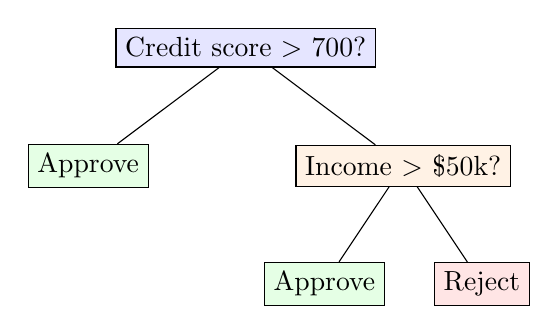
\begin{tikzpicture}[level distance=1.5cm,
      level 1/.style={sibling distance=4cm},
      level 2/.style={sibling distance=2cm}]
    \node[draw, rectangle, fill=blue!10] {Credit score $>$ 700?}
      child {node[draw, rectangle, fill=green!10] {Approve}}
      child {node[draw, rectangle, fill=orange!10] {Income $>$ \$50k?}
        child {node[draw, rectangle, fill=green!10] {Approve}}
        child {node[draw, rectangle, fill=red!10] {Reject}}
      };
    \end{tikzpicture}
    \end{center}

%\textbf{Split Criteria}

%Classification: split so that \text{Gini impurity} is minimized
%\[
%\text{Gini} = 1 - \sum_k p_k^2
%\]

%Regression:
%    A decision tree is a model that predicts outcomes by recursively splitting data based on feature values, forming a tree of decisions. Each internal node tests a feature, and each leaf gives a prediction. Decision trees are interpretable and visualize how decisions are made.
\end{frame}
\begin{frame}{Random Forest: Main Idea}

\textbf{Instead of one tree:}

\[
\text{Build many trees}
\]

\vspace{0.4cm}

\textbf{Each tree}

\begin{itemize}
    \item Trained on subset sample of data
    \item Uses random subset of features at each split
\end{itemize}

\vspace{0.4cm}

\textbf{Aggregation}

\begin{itemize}
    \item Regression $\rightarrow$ average prediction
    \item Classification $\rightarrow$ majority vote
\end{itemize}

\end{frame}
\begin{frame}{Introduction to Neural Networks}

One hidden layer network:

\[
h(x) = W\sigma(w_0+w_1x_1+\cdots + w_px_p)+b_2
\]

\vspace{0.4cm}

\textbf{Key idea}

\begin{itemize}
    \item Linear transformations
    \item Followed by nonlinear activation
\end{itemize}

\vspace{0.3cm}

Universal function approximator when sufficiently large.

\end{frame}
\begin{frame}[fragile]{Neural networks: multilayer perceptron regression}

 $1$- layer perceptron with hidden layer of size $1$ with one output
       \[ 
          \begin{split}
            g(x_1,\ldots,x_n)=W_2 \sigma(W_1 x + b_1)+b_2 = \\
           W_2\sigma(W_{11}x_1+\cdots + W_{1n}x_n+b_1)+b_2 
         \end{split}
      \]


$\sigma$ -- activation function: 

\begin{itemize}
\item hyperbolic tangent:   $\sigma(x)=\frac{e^x-e^{-x}}{e^x+e^{-x}}$ 

\item logistic function:  $\sigma(x)=\frac{1}{1+e^{-x}}$

\item linear:  $\sigma(x)=x$

\item RELU $\sigma(x)=\max(0,x)$. 

\end{itemize}

 $W_2,b_1,b_2$ scalars, $W_1=(W_{11},\ldots,W_{1n})$ 


\end{frame}
\begin{frame}[fragile]{Neural networks: multilayer perceptron regression}

	$1$- layer perceptron with hidden layer of size $1$ with one output ($1$-neuron neural network)
	 \begin{figure}
\begin{center}
\begin{tikzpicture}
 %%\tikzstyle{mode}=[draw,transform shape, minimum size=10mm]
	\draw (12,6)++(15,5) node{Neuron};
  \node[draw,right, text centered, text width=20ex,transform shape, minimum size = 15mm] at 
  (0,0) (SW) 
	{linear regression};
	\node[draw,right, text centered, text width=20ex,transform shape, minimum size = 15mm] 
	at (30,0)  (ACT) {$\hat{y}=\sigma(W\hat{y}_1+b_2)$};
	\draw[->] (ACT.east)++(0,0) -- ++(5,0) node[pos=0.3]{$\hat{y}$};
	\draw[->] (SW.east)++(0,0) -- (ACT.west) node[pos=0.3]{$\hat{y}_1$};
  %\draw[<-] (SW.west)++(0,3) -- ++(-8,3); % node{$x_1$};
	\node[draw,circle] at (-8,12) (X1) {$x_1$};
	\node[draw,circle] at (-8,6) (X2) {$x_2$};
	\node  at (-8,0) (Xst) {$\vdots$};
	\node[draw,circle] at (-8,-8) (Xn) {$x_n$};
	 \draw[<-] (SW.west)++(0,3) -- (X1);
	 \draw[<-] (SW.west)++ (0,2)-- (X2);
	 \draw[<-] (SW.west)++(0,-2) -- (Xn);
  %\draw  (SW.west)++(-8,5) node{$x_1$};
  %\draw[<-] (SW.west)++(0,2) -- ++(-8,2); % node{$x_2$};
  %\draw  (SW.west)++(-8,1) node{$x_2$};
  %\draw[<-] (SW.west)++(0,0) -- ++(-5,0); % node[pos=0.2]{$\vdots$};
  %\draw[<-] (SW.west)++(0,-3) -- ++(-8,-3);% node{$x_n$};
  %\draw  (SW.west)++(-8,-4) node{$x_n$};
\end{tikzpicture}
\end{center}
\end{figure}


%       \[ 
%          \begin{split}
%            g(x_1,\ldots,x_n)=%W_2 \sigma(W_1 x + b_1)+b_2 = \\
%           W_2\sigma(W_{11}x_1+\cdots + W_{1n}x_n+b_1)+b_2 
%         \end{split}
%      \]
%
%	$W_2, W_{11} \ldots, W_{1n}$ -- weights, $b_1,b_2$ --  biases. 

$\sigma$ -- activation function: 

\begin{itemize}
\item hyperbolic tangent:   $\sigma(x)=\frac{e^x-e^{-x}}{e^x+e^{-x}}$ 

\item logistic function:  $\sigma(x)=\frac{1}{1+e^{-x}}$

\item linear:  $\sigma(x)=x$

\item RELU $\sigma(x)=\max(0,x)$. 

\end{itemize}

% $W_2,b_1,b_2$ scalars, $W_1=(W_{11},\ldots,W_{1n})$ 


\end{frame}
\begin{frame}[fragile]{Neural networks: multilayer perceptron regression}


	$1$- layer perceptron with hidden layer of size $k$  ($k$ neurons) and with one output

\begin{figure}
 \begin{center}
	 \begin{tikzpicture}[scale=0.7]
 %%\tikzstyle{mode}=[draw,transform shape, minimum size=10mm]
  \node[draw,right, text centered, text width=20ex,transform shape, minimum size = 15mm] at 
  (0,10) (SW1) 
	{linear regression 1};
    \node[draw,right, text centered, text width=20ex,transform shape, minimum size = 15mm] at 
  (60,0) (SWf) 
	{final linear regression};
	\draw (SW1.north)++(15,3) node{Neuron  1};
  \node[draw,right, text centered, text width=20ex,transform shape, minimum size = 15mm] at 
  (0,-10) (SWk) 
	{linear regression k};
  	\draw (SWk.north)++(15,3) node{Neuron k};
  %\node[draw,right, text centered, text width=20ex,transform shape, minimum size = 15mm] at 
  %(0,-20) (SWk) 
	{linear regression $k$};
	%\draw (SWk.north)++(0,3) node{Hidden layer $k$};
	\node[draw,right, text centered, text width=15ex,transform shape, minimum size = 15mm] 
	at (30,10)  (ACT1) {$\hat{y}_1=\sigma(\hat{h}_1)$};
		\node[draw,right, text centered, text width=15ex,transform shape, minimum size = 15mm] 
	at (30,-10)  (ACTk) {$\hat{y}_k=\sigma(\hat{h}_k)$};

	\draw[->] (ACT1) -- (SWf) node[pos=0.3]{$\hat{y}_1$};
	\draw[->] (ACTk) -- (SWf) node[pos=0.3]{$\hat{y}_k$};
	\draw[->] (SW1) -- (ACT1) node[pos=0.3]{$\hat{h}_1$};
	\draw[->] (SWk) -- (ACTk) node[pos=0.3]{$\hat{h}_1$};
	\draw[->] (SWf.south) -- ++(0,-5) node[pos=0.3]{$\hat{y}$};
  %\draw[<-] (SW.west)++(0,3) -- ++(-8,3); % node{$x_1$};
	\node[draw,circle] at (-8,12) (X1) {$x_1$};
	\node[draw,circle] at (-8,6) (X2) {$x_2$};
	\node  at (-8,0) (Xst) {$\vdots$};
	\node  at (30,0) (Hst) {$\vdots$};
	\node  at (10,0) (Hst2) {$\vdots$};
	\node[draw,circle] at (-8,-8) (Xn) {$x_n$};

	 \draw[<-] (SW1) -- (X1);
	 \draw[<-] (SW1)-- (X2);
	 \draw[<-] (SW1) -- (Xn);
	  \draw[<-] (SWk) -- (X1);
	 \draw[<-] (SWk)-- (X2);
	 \draw[<-] (SWk) -- (Xn);

  %\draw  (SW.west)++(-8,5) node{$x_1$};
  %\draw[<-] (SW.west)++(0,2) -- ++(-8,2); % node{$x_2$};
  %\draw  (SW.west)++(-8,1) node{$x_2$};
  %\draw[<-] (SW.west)++(0,0) -- ++(-5,0); % node[pos=0.2]{$\vdots$};
  %\draw[<-] (SW.west)++(0,-3) -- ++(-8,-3);% node{$x_n$};
  %\draw  (SW.west)++(-8,-4) node{$x_n$};
\end{tikzpicture}
\end{center}
\end{figure}




       %\[ \begin{split} 
%	       g(x_1,\ldots,x_n)&=W_{2,1} y_1+\cdots + W_{2,k} y_k +b_2 \\
	%W_2 \stackrel{\rightarrow}{\sigma}(W_1 x + b_1)+b_2 =  \\
%	       y_1&=\sigma(W_{1,1}x_1+\cdots W_{1,n}x_n)+b_{1,1}  \mbox{ output first layer }  \\
%	       y_2&=\sigma(W_{2,1}x_1+\cdots W_{2,n}x_n)+b_{2,1}  \mbox{ output second layer }\\
%	       \vdots & \vdots \\
%	       y_k& =\sigma(W_{k,1}x_1+\cdots W_{k,n}x_n)+b_{k,1} \mbox{ output $k$th layer }\\
%       \end{split}
%       \]

 %$W_2,b_2$ scalars, 

 %\medskip

 %$W_1=\begin{bmatrix} W_{11}^1 & \cdots & W_{1n}^1  \\   W_{21}^1 & \cdots & W_{2n}^1 \\ \vdots & \cdots & \vdots \\ W_{k1}^1 & \cdots & W_{kn}^1 \end{bmatrix}$, 
  %$b_1=\begin{bmatrix} b_{1,1} \\ \vdots \\ b_{1,k} \end{bmatrix}$, $\stackrel{\rightarrow}{\sigma}(\begin{bmatrix} z_1 \\ \vdots \\ z_k \end{bmatrix})=\begin{bmatrix} \sigma(z_1) \\ \vdots \\ \sigma(z_k) \end{bmatrix}$

\end{frame}

 %$2$ - layer perceptron

%       \[ g(x_1,\ldots,x_n)=W_3\stackrel{\rightarrow}{\sigma}(W_2 \stackrel{\rightarrow}{\sigma}(W_1x+b_1) + b_2)+b_3 \]
 

\begin{frame}[fragile]{Neural networks: multilayer perceptron regression}

Cascade of several 1-layer nerual networks: output of one 1-layer neural network is the input of the next one.

 \begin{center}
 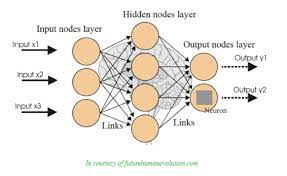
\includegraphics[scale=0.7]{index.jpeg}
 \end{center}

\end{frame}
%\begin{frame}[fragile]{Neural networks: multilayer perceptron regression}

% $N$ -layer perceptron, $N$ hidden layers, $i$th hidden layer of size $k_i$, $p$ outputs
%
%       \[ g(x_1,\ldots,x_n)=W_N(\stackrel{\rightarrow}{\sigma} (W_{N-1} \stackrel{\rightarrow}{\sigma} ( \cdots \stackrel{\rightarrow}{\sigma}(W_1x+b_1) + b_2) \cdots + b_{N-1})+b_N \]
%

% \bigskip 

%  $W_i$ matrices of size $k_{i+1} \times k_i$, $i=2,\ldots,N-1$, and $W_1$ is a matrix of size $k_1 \times n$  and $W_N$ is a matrox of size $p \times k_N$.

%  \medskip

%  $b_i$ vectors of size $k_{i} \times 1$, $i=1,\ldots,N-1$, $b_N$ vector of size $p \times 1$. 

% \medskip

%  $p$ -- number of outputs, $n$ is the number of inputs, $k$ is the size of each layer.

% \medskip

%  $W_1,\ldots,W_N$ weights, $b_1,\ldots,b_N$ bias vectors


% \medskip

% Loss function: $\mathbf{l}(y,\hat{y})=\sum_{i=1}^{p} (y_i-\hat{y}_i)^2$






%\end{frame}
\begin{frame}[fragile]{Neural networks: multilayer perceptron regression}

 \lstinline$from sklearn.neural_network import MLPRegressor$


 \begin{lstlisting}

 nw=MLPRegressor(hiden_layer_sizes=(k_1,k_2,...,k_N), 
          activation=func, max_iter=iter)


 \end{lstlisting}


 \bigskip

 \begin{itemize}
 \item \lstinline$k_1,...,k_N$ sizes of the first, second, etc. $N$th layer.

 \medskip

 \item \lstinline$func$ can be \lstinline$'identity'$, \lstinline$'logistic'$,  \lstinline$'tanh'$, \lstinline$'relu'$.
 
 \medskip

  \item \lstinline$iter$ the bigger the number is, the more likely to find optimal model.
	  %$W_1,\ldots,W_N,b_1,\ldots,b_N$ which 
%  minimizes the loss function. 

  
 \end{itemize}


 \lstinline$nw.fit(X_train,y_train)$, \lstinline$nw.predict(X_test)$. 

 



\end{frame}


% =====================================================
\section{Module 6 — Machine Learning in Practice}

\begin{frame}{Module 6 — ML in Practice}
\begin{itemize}
    \item Feature Engineering
    \item Train / Validation / Test Split
    \item Cross-Validation
    \item Practical ML Pipeline
    \item Model Monitoring
    \item Hypothesis Testing for Model Drift
\end{itemize}
\end{frame}

\begin{frame}{Business Example: Raw Data Is Not Enough}

Suppose we predict house prices.

Available variables:

\begin{itemize}
    \item Size (m$^2$)
    \item Year built
    \item Zip code
\end{itemize}

\vspace{0.5cm}

Question:

Should we use them directly?

\end{frame}

\begin{frame}{Feature Engineering}

Feature engineering:

\[
\text{Transform raw data into informative variables}
\]

\vspace{0.5cm}

Examples:

\begin{itemize}
    \item Age of house = Current year - Year built
    \item One-hot encoding of zip code
    \item Interaction: Size $\times$ Location
    \item Log-transform price
\end{itemize}

\vspace{0.5cm}

Better features $\rightarrow$ Better models

\end{frame}

\begin{frame}{Common Feature Transformations}

\begin{itemize}
    \item Scaling (standardization)
    \[
    x' = \frac{x - \mu}{\sigma}
    \]

    \item Min-Max scaling
    \[ x' = \frac{x - \min(x)}{\max(x) - \min(x)} \]

    \item Log-transform for skewed variables

    \item Polynomial features

    \item Categorical encoding (one-hot)
\end{itemize}

\vspace{0.5cm}

Important for:

\begin{itemize}
    \item Linear models
    \item Regularization
    \item Gradient descent
\end{itemize}

\end{frame}

\begin{frame}{Why Train/Test Split?}

Suppose our model achieves:

\[
R^2 = 0.95
\]

on training data.

\vspace{0.5cm}

Question:

Will it perform equally well on new customers?

\end{frame}

\begin{frame}{Train / Validation / Test Split}

Dataset is divided into:

\begin{itemize}
    \item Training set → Fit model
    \item Validation set → Tune hyperparameters
    \item Test set → Final unbiased evaluation
\end{itemize}

\vspace{0.5cm}

Important:

\[
\text{Test set must not influence model choice}
\]

\end{frame}

\begin{frame}{Cross-Validation}

Instead of one split:

\[
\text{Use multiple splits}
\]

\vspace{0.5cm}

K-fold cross-validation:

\begin{itemize}
    \item Split data into K folds
    \item Train on K-1 folds
    \item Validate on remaining fold
    \item Repeat K times
\end{itemize}

\vspace{0.5cm}

Provides more stable performance estimate.

\end{frame}

\begin{frame}{Business Problem: Model Drift}

Suppose churn model was deployed 6 months ago.

\vspace{0.5cm}

Question:

Has customer behavior changed?

\vspace{0.5cm}

If distribution changes:

\[
P_{\text{train}}(X) \neq P_{\text{production}}(X)
\]

Model performance may degrade.

\end{frame}

\begin{frame}{Monitoring with Hypothesis Testing}

We test:

\[
H_0: \text{Distribution unchanged}
\]

\[
H_1: \text{Distribution changed}
\]

\vspace{0.5cm}

Example tests:

\begin{itemize}
    \item t-test (mean change)
    \item Kolmogorov–Smirnov test
    \item Chi-square test (categorical)
\end{itemize}

\end{frame}

\begin{frame}{Monitoring Model Performance}

We monitor metrics over time:

\begin{itemize}
    \item Accuracy
    \item Precision / Recall
    \item $R^2$
\end{itemize}

\vspace{0.5cm}

Hypothesis test:

\[
H_0: \text{Performance unchanged}
\]

\vspace{0.3cm}

If rejected:

\begin{itemize}
    \item Retrain model
    \item Update features
    \item Re-evaluate pipeline
\end{itemize}

\end{frame}

\begin{frame}{Typical ML Pipeline}

\begin{enumerate}
    \item Data collection
    \item Feature engineering
    \item Train/Validation split
    \item Model training
    \item Hyperparameter tuning
    \item Final evaluation on test set
    \item Deployment
\end{enumerate}

\vspace{0.5cm}

Machine learning is an iterative process.

\end{frame}
% =====================================================
\section{Module 4 — Generalization and Model Evaluation}

\begin{frame}{Module 4 — Generalization}
\begin{itemize}
    \item Overfitting vs Underfitting
    \item Bias–Variance Tradeoff
    \item Regularization (L1 and L2)
    \item Decision Boundaries
    \item Performance Metrics:
    \begin{itemize}
        \item R\textsuperscript{2}
        \item Accuracy
        \item Precision
        \item Recall
        \item F1-score
    \end{itemize}
\end{itemize}
\end{frame}

\begin{frame}{Overfitting vs Underfitting}

\textbf{Problem:} How well does a model generalize to unseen data?

\vspace{0.5cm}

\begin{itemize}
    \item \textbf{Underfitting:} Model is too simple
    \begin{itemize}
        \item Fails to capture patterns in training data
        \item High bias, low variance
        \item Poor performance on both training and test sets
        \item Example: Linear model trying to fit a quadratic trend
    \end{itemize}
    \item \textbf{Overfitting:} Model is too complex
    \begin{itemize}
        \item Captures noise as if it were signal
        \item Low bias, high variance
        \item Excellent performance on training set, poor on test set
        \item Example: High-degree polynomial for limited data points
    \end{itemize}
\end{itemize}

\vspace{0.5cm}

\textbf{Business Example:}  
A pricing model fits historical sales perfectly (overfit) but predicts future sales poorly.

\end{frame}

\begin{frame}{Bias--Variance Tradeoff}

\textbf{Problem:} Why does increasing model complexity sometimes hurt performance?

\vspace{0.5cm}

Prediction error can be decomposed into:

\[
\text{Error}
=
\text{Bias}^2
+
\text{Variance}
+
\text{Noise}
\]

\begin{itemize}
    \item \textbf{Bias:} Error from overly simple assumptions  
    High bias $\rightarrow$ underfitting
    \item \textbf{Variance:} Sensitivity to small fluctuations in training data  
    High variance $\rightarrow$ overfitting
    \item \textbf{Noise:} Irreducible randomness in the data
\end{itemize}

\vspace{0.5cm}

\textbf{Business Example:}  
A very simple demand model ignores seasonality (high bias).  
A very complex model reacts to random weekly fluctuations (high variance).

\end{frame}

\begin{frame}{Regularization}

\textbf{Goal:} Prevent overfitting by controlling model complexity.

\vspace{0.5cm}

General form of regularized loss:

\[
L(\mathbf{w})
=
\sum_{i=1}^n (y_i - \mathbf{w}^T x_i)^2
+
\lambda \Omega(\mathbf{w})
\]

\begin{itemize}
    \item $\lambda$ controls the strength of the penalty
    \item Larger $\lambda$ $\rightarrow$ simpler model
\end{itemize}

\vspace{0.3cm}

\begin{tabular}{c|c|c}
Method & Penalty & Effect \\
\hline
Ridge (L2) & $\sum w_j^2$ & Shrinks coefficients \\
Lasso (L1) & $\sum |w_j|$ & Produces sparse model
\end{tabular}

\vspace{0.5cm}

\textbf{Business Example:}  
In marketing analytics with 100 features, regularization avoids unstable and extreme coefficient estimates.

\end{frame}

\begin{frame}{Decision Boundary in Logistic Regression}

\textbf{Goal:} Understand how logistic regression separates classes.

\vspace{0.5cm}

Prediction rule:

\[
Y = 1 
\quad \text{if} \quad 
\sigma(w^T x) > 0.5
\]

This is equivalent to:

\[
w^T x = 0
\]

\begin{itemize}
    \item The equation defines a \textbf{hyperplane}
    \item Points on one side $\rightarrow$ Class 1
    \item Points on the other side $\rightarrow$ Class 0
\end{itemize}

\vspace{0.5cm}

\textbf{Business Example:}  
In credit scoring, the decision boundary separates high-risk from low-risk applicants based on their features.

\end{frame}

\begin{frame}{Regression Metrics}

\begin{itemize}
    \item \textbf{R\textsuperscript{2} (Coefficient of Determination):}
    \[
    R^2 = 1 - \frac{\sum_{i=1}^n (y_i - \hat{y}_i)^2}{\sum_{i=1}^n (y_i - \bar{y})^2}
    \]
    Indicates proportion of variance explained by the model. $R^2 \approx 1$ is good.
    
    \item \textbf{Mean Squared Error (MSE):}
    \[
    \text{MSE} = \frac{1}{n} \sum_{i=1}^n (y_i - \hat{y}_i)^2
    \]
    Penalizes large errors more heavily.
    
    \item \textbf{Mean Absolute Error (MAE):}
    \[
    \text{MAE} = \frac{1}{n} \sum_{i=1}^n |y_i - \hat{y}_i|
    \]
    Robust to outliers; measures average absolute deviation.
\end{itemize}

\end{frame}

\begin{frame}{Classification Metrics - Part 1}

\begin{itemize}
    \item \textbf{Accuracy:} Fraction of correct predictions
    \[
    \text{Accuracy} = \frac{TP + TN}{TP + TN + FP + FN}
    \]
    Simple overall measure, but can be misleading for imbalanced classes.
    
    \item \textbf{Precision:} Fraction of positive predictions that are correct
    \[
    \text{Precision} = \frac{TP}{TP + FP}
    \]
    Important when false positives are costly.
\end{itemize}

\end{frame}

\begin{frame}{Classification Metrics - Part 2}

\begin{itemize}
    \item \textbf{Recall (Sensitivity):} Fraction of actual positives correctly identified
    \[
    \text{Recall} = \frac{TP}{TP + FN}
    \]
    Important when missing a positive is costly.
    
    \item \textbf{F1-score:} Harmonic mean of Precision and Recall
    \[
    F1 = 2 \cdot \frac{\text{Precision} \cdot \text{Recall}}{\text{Precision} + \text{Recall}}
    \]
    Balances precision and recall.
\end{itemize}

\end{frame}

\end{document}

% =====================================================


% =====================================================
\section{Module 7 — Unsupervised Learning}

\begin{frame}{Module 7 — Clustering}
\begin{itemize}
    \item Introduction to Clustering
    \item K-Means Algorithm
    \item Importance of Distance Metrics
    \item Silhouette Score
\end{itemize}
\end{frame}

\begin{frame}{Business Example: Customer Segmentation}

Suppose we have customer data:

\begin{itemize}
    \item Annual income
    \item Spending score
\end{itemize}

\vspace{0.5cm}

Goal:

\[
\text{Group customers into segments}
\]

\vspace{0.5cm}

No labels are available.

\end{frame}

\begin{frame}{What is Clustering?}

Clustering is an unsupervised learning task.

\vspace{0.5cm}

Given data points:

\[
x_1, \dots, x_n
\]

Partition them into $K$ groups such that:

\begin{itemize}
    \item Points in same cluster are similar
    \item Points in different clusters are dissimilar
\end{itemize}

\end{frame}

\begin{frame}{K-Means Algorithm}

Choose number of clusters $K$.

\vspace{0.5cm}

Goal:

\[
\min_{C_1,\dots,C_K}
\sum_{k=1}^K
\sum_{x_i \in C_k}
\|x_i - \mu_k\|^2
\]

\vspace{0.5cm}

Where:

\[
\mu_k = \text{mean of cluster } C_k
\]

\end{frame}

\begin{frame}{K-Means: Algorithm Steps}

\begin{enumerate}
    \item Initialize $K$ centroids randomly
    \item Assign each point to closest centroid
    \item Update centroids (compute cluster means)
    \item Repeat until convergence
\end{enumerate}

\vspace{0.5cm}

Convergence:

\begin{itemize}
    \item Assignments stop changing
    \item Centroids stabilize
\end{itemize}

\end{frame}

\begin{frame}{Importance of Distance}

K-means relies on distance:

\[
\|x_i - \mu_k\|
\]

\vspace{0.5cm}

Typically:

\[
\text{Euclidean distance}
\]

\vspace{0.5cm}

Implications:

\begin{itemize}
    \item Features must be scaled
    \item Sensitive to outliers
    \item Assumes spherical clusters
\end{itemize}

\end{frame}

\begin{frame}{Why Feature Scaling is Crucial}

Suppose we cluster customers using:

\begin{itemize}
    \item Income (0–100,000)
    \item Spending score (0–100)
\end{itemize}

\vspace{0.5cm}

Without scaling:

\[
\text{Income dominates distance}
\]

\vspace{0.5cm}

Solution:

\[
x' = \frac{x - \mu}{\sigma}
\]

\end{frame}

\begin{frame}{Choosing the Number of Clusters}

Key question:

\[
\text{What is the optimal } K?
\]

\vspace{0.5cm}

Common methods:

\begin{itemize}
    \item Elbow method
    \item Silhouette score
\end{itemize}

\end{frame}

\begin{frame}{Silhouette Score}

For each point:

\begin{itemize}
    \item $a$ = average distance to points in same cluster
    \item $b$ = smallest average distance to other clusters
\end{itemize}

\vspace{0.5cm}

Silhouette value:

\[
s = \frac{b - a}{\max(a, b)}
\]

\end{frame}

\begin{frame}{Interpretation of Silhouette Score}

\[
-1 \leq s \leq 1
\]

\vspace{0.5cm}

\begin{itemize}
    \item $s \approx 1$ → well clustered
    \item $s \approx 0$ → overlapping clusters
    \item $s < 0$ → likely misclassified
\end{itemize}

\vspace{0.5cm}

Overall quality:

\[
\text{Average silhouette score}
\]

\end{frame}

\begin{frame}{Business Interpretation}

High silhouette score:

\begin{itemize}
    \item Clear customer segments
    \item Targeted marketing possible
\end{itemize}

\vspace{0.5cm}

Low silhouette score:

\begin{itemize}
    \item Segments overlap
    \item Clustering may not be meaningful
\end{itemize}

\vspace{0.5cm}

Clustering must be both:

\[
\text{Mathematically sound and business relevant}
\]

\end{frame}


% =====================================================
\section{Conclusion}

\begin{frame}{Conclusion}
\begin{itemize}
    \item From Probability to Business Decisions
    \item Choosing the Right Model
    \item The Complete ML Pipeline
    \item Responsible and Monitored Deployment
\end{itemize}
\end{frame}


\end{document}
